\documentclass[11pt]{book}
\usepackage[top=1.5in,left=1.0in,right=1.0in,bottom=1.5in]{geometry}
\usepackage{amsmath,amsthm,amssymb,amsfonts,enumerate}
\usepackage[utf8]{inputenc}
\usepackage[spanish]{babel}
\usepackage{hyperref}
\usepackage[pdftex]{graphicx}
\usepackage{color}

\usepackage{biblatex}
\bibliography{thesis.bib}

\setlength{\parindent}{0cm}
\setlength{\parskip}{0.3cm}

\theoremstyle{definition}
\newtheorem{definition}{Definición}
\numberwithin{definition}{section}

\makeatletter
\def\th@definition{ \thm@notefont{} \thm@headpunct{.\\} }
\def\th@theorem{ \thm@notefont{} \thm@headpunct{.\\} }
\def\th@plain{ \thm@notefont{\normalfont} \thm@headpunct{.\\} }
\makeatother

\theoremstyle{theorem}
\newtheorem{theorem}{Teorema}
\newtheorem{lemma}{Lema}
\newtheorem{proposition}{Proposición}
\newtheorem{corollary}{Corolario}
\numberwithin{theorem}{section}
\numberwithin{lemma}{section}
\numberwithin{corollary}{section}

\theoremstyle{plain}
\newtheorem{example}{Ejemplo}
\numberwithin{example}{section}
\newtheorem{remark}{Nota}

\renewcommand\qedsymbol{$\blacksquare$}

\newcommand{\N}{{\ensuremath{\mathbb{N}}}}
\newcommand{\Z}{{\ensuremath{\mathbb{Z}}}}
\newcommand{\Q}{{\ensuremath{\mathbb{Q}}}}
\newcommand{\R}{{\ensuremath{\mathbb{R}}}}
\newcommand{\C}{{\ensuremath{\mathbb{C}}}}
% \newcommand{\vect}[1]{\vec{#1}} % vectors

\begin{document}

\title{Sistemas Dinámicos Planos}
\author{Jorge A. Torres H.}
\maketitle

\tableofcontents

\chapter{Introducción}
\label{cap:introduccion}

...

\chapter{Sistemas Dinámicos Planos}
\label{cap:sistemasplanosautonomos}

\section{Conceptos Básicos}

\begin{definition}[Sistema Dinámico Plano] \label{def:dynamicalsystem}
Sean $T \subseteq \R$ un semigrupo aditivo, $X$ un subconjunto de $\R^2$ y $\phi: T \times X \to X: (t,x) \mapsto \phi^t(x)$ una función. Un \emph{sistema dinámico plano} es una tupla $(T, X, \phi)$ que satisface las propiedades

\begin{enumerate}[(1)]
    \item $\phi \left( 0, x \right) = \phi \left( x \right)$ para todo $x \in
    X$. Equivalentemente $\phi^0 \equiv \text{id}_X$.
    
    \item $\phi \left( t, \phi \left( s, x \right) \right) = \phi \left(
    s + t, x \right)$ para todo $x \in X$ y $s, t \in T$. Equivalentemente $\phi^{s} \circ \phi^{t} \equiv \phi^{s + t}$.
\end{enumerate}

El conjunto $T$ se llama \emph{espacio de tiempos}, $X$ es llamado {\emph{espacio de estados (o de fase)}} y $\phi$ se conoce como {\emph{operador de evoluci\'on}}.
\end{definition}

Se puede pensar en un operador de evolución $\phi$ como una colección de funciones $\{ \phi^t: X \to X \}_t$, llamada también \emph{flujo}, que ``mueve'' un punto $x_0$ por el estado de fases $X$ a través de la curva $t \mapsto \phi^t(x_0)$ como en la figura \ref{fig:evolutionoperator}.

\begin{remark}
Un sistema dinámico se dice \emph{discreto} si el espacio de tiempos $T$ es discreto ($T \subseteq \Z$). En caso contrario, se dice \emph{continuo}.
\end{remark}

\begin{remark}
A menudo el operador de evolución $\phi$ no está definido en todo $T \times X$ sino en un subconjunto $U \subseteq T \times X$. En tal caso pedimos que $\{ 0 \} \times X \subseteq U$ y que las propiedades (1) y (2) de la definición \ref{def:dynamicalsystem} se satisfagan siempre que $(t, x)$ esté en $U$.

Es decir, dado $x \in X$ existe un subconjunto de tiempo (usualmente un intervalo) $I_x := \{ t \in T : (t,x) \in U \} \subseteq T$ tal que $\phi(t,x)$ está definida para todo $t \in I_x$.
\end{remark}

\begin{figure}[!ht] \label{fig:evolutionoperator} \centering
    \includegraphics[scale=1.3]{figures/evolution-operator.pdf}
    \caption{Operador de evolución.}
\end{figure}

En lo que sigue supondremos que $( T, X, \phi )$ es un sistema
dinámico.

Dado un $x_0 \in X$, un estado inicial, deseamos estudiar la geometr\'{\i}a del
conjunto de todos los posibles estados futuros y pasados del sistema
din\'amico, obtenidos a partir de $x_0$ haciendo uso del operador de
evoluci\'on $\phi$.
Para tal fin introducimos el concepto de órbita.

\begin{definition}
  \label{def:orbit}La {\emph{\'orbita (o trayectoria) positiva
  $\gamma^+_{x_0}$}}, {\emph{\'orbita negativa $\gamma^-_{x_0}$}} y
  {\emph{\'orbita $\gamma_{x_0}$}} de $x_0$ (o a trav\'es de $x_0$) son
  los subconjuntos del espacio de estados $X$, definidos por
  \[ \gamma^+_{x_0} := \left\{ \phi \left( t, x \right) : t \in I_{x_0},
     t \geq 0 \right\} = \left\{ \phi^t \left( x_0 \right) \right\}_{t
     \in I_{x_0}, t \geq 0}, \]
  \[ \gamma^-_{x_0} := \left\{ \phi^t \left( x_0 \right) \right\}_{t \in
     I_{x_0}, t \leq 0}, \]
  \[ \gamma_{x_0} := \gamma_{x_0}^+ \cup \gamma_{x_0}^- = \left\{ \phi
     \left( t, x \right) : t \in I_{x_0} \right\} = \left\{ \phi^t \left( x_0
     \right) \right\}_{t \in I_{x_0}} . \]
  Una \'orbita que consiste de un solo punto se llama {\emph{\'orbita
  constante}}.
\end{definition}

Mientras que las \'orbitas de un sistema din\'amico continuo son curvas en el
espacio $M$ parametrizadas por $t$ y orientadas en la direcci\'on de
crecimiento, las de un sistema din\'amico discreto son sucesiones de puntos
$\ldots ., f^{- 1} \left( x_0 \right), x_0, f \left( x_0 \right), f^2 \left(
x_0 \right), \ldots$ indizadas por enteros, como en la figura \ref{fig:orbits}.

\begin{figure}[ht] \centering \label{fig:orbits}
    \includegraphics[scale=1.3]{figures/orbits-continuousanddiscrete.pdf}
    \caption{Órbitas en un sistema dinámico continuo y uno discreto.}
\end{figure}

\begin{definition}
  \label{def:equilibrium}Un punto $x \in X$ es un {\emph{equilibrio}} (o
  {\emph{punto fijo o punto crítico}}) si $\gamma_x = \left\{ x \right\}$ (es decir,
  $\phi^t \left( x \right) = x$ para todo $t \in T$).
\end{definition}

Lo anterior implica que un sistema din\'amico puesto en un equilibrio permanece all\'{\i} por siempre. Rec\'{\i}procamente, las \'orbitas constantes corresponden a equilibrios del sistema.

\begin{definition}
  \label{def:periodicorbit}Una {\emph{\'orbita peri\'odica (o ciclo) $O$}}
  es una \'orbita no constante para la cual existe $t_0 \in T$ tal que
  $\phi^{t + t_0} \left( x_0 \right) = \phi^t \left( x_0 \right)$ para todo $t
  \in T$ y $x_0 \in O$.
  
  El m\'{\i}nimo $t_0$ que satisface lo anterior se llama
  {\emph{per\'{\i}odo de la \'orbita.}}
\end{definition}

Esto es, si el sistema din\'amico evoluciona desde un $x_0$ en un ciclo $O$,
regresar\'a exactamente a este punto $x_0$ a las $t_0$ unidades de tiempo. Por
tanto, una \'orbita peri\'odica de un sistema continuo es una curva
{\emph{cerrada}} en el espacio de fase.

\begin{figure}[!hb] \label{fig:cycle} \centering
    \includegraphics[scale=1.3]{figures/orbit-cycle.pdf}
    \caption{Una órbita periódica (ciclo) $O$ a través de $x_0$.}
\end{figure}

\begin{definition}[Diagrama de Fase]
  \label{def:phasediagram}Al dibujar la colecci\'on de todas las \'orbitas
  (con sus direcciones) obtenemos un {\emph{diagrama de fase}}.
\end{definition}
En la pr\'actica, solo unas \'orbitas representativas son consideradas en el diagrama de fase.

\begin{example}[Mapa Logístico]
Aunque se trata de un sistema unidimensional ($X \subseteq \R$) este es un buen ejemplo introductorio a la temática de sistemas dinámicos.

El mapa logístico es una relación de recurrencia no lineal popularizada por Robert May \cite{may76} como modelo demográfico de tiempo discreto.
Supongamos que existe un número máximo posible para los individuos de cierta población y sea $x_n \in [0,1]$ la fracción de dicho máximo de individuos que hay en el año $n$ en la población. Si $r$ es la tasa combinada de reproducción y mortandad de la población, el mapa logístico corresponde a la expresión

\begin{equation} \label{eq:mapalogistico}
x_{n+1} = rx_n(1-x_n).
\end{equation}

La ecuación \ref{eq:mapalogistico} está relacionada con dos fenómenos demográficos: el crecimiento es proporcional a la población existente $x_n$ cuando dicha población es pequeña. Existe, sin embargo, un valor crítico para el cual la tasa de mortalidad supera a la de crecimiento.
Esto pues $x_n^2$ es pequeño en comparación a $x_n$ cuando $x_n$ es pequeño pero este comportamiento se reversa una vez $x_n > 1$.

El mapa logístico puede entenderse como un sistema dinámico discreto con espacio de tiempo $T = \Z$, espacio de fase $X = [0,1]$ y operador de evolución dado por

\begin{equation} \label{eq:evolucionmapalogistico}
	\phi(n + 1, x) = x_{n+1} = rx_n(1-x_n).
\end{equation}

El sistema tiene un punto de equilibrio trivial en $x = 0$ pues $\phi^n(0) = 0$ para todo $n \in \Z$. Hay otro punto de equilibrio en $x = (r-1)/r$ pues

$$ \phi^1((r-1)/r) = r \frac{r-1}{r} \left(1 - \frac{r-1}{r} \right) = (r-1) \left( \frac{r - r + 1}{r} \right) = \frac{r-1}{r}. $$

El caso $r = 4$ es de particular interés pues presenta comportamiento caótico \cite[p.~19]{fractallectures} y porque la relación de recurrencia puede solucionarse de manera explícita \cite{lorenz64} como

$$  \phi^n(x) = \sin^2( 2^n \sin^{-1}( x^{1/2} ) ). $$

Algunas órbitas convergen al punto crítico $x = 0$ luego de un número finito de iteraciones pero la mayoría presentan un comportamiento errático. Por ejemplo, la órbita de $x = 1/2$ es $\gamma^+(1/2) = \{ 1/2, 1, 0, 0, 0, 0, ... \}$ mientras que las órbitas de $x = 0.6$ y $x = 0.61$, dos números muy cercanos, divergen en pocas iteraciones la una de la otra:

$$
	\begin{array}{lll}
		\gamma^+(0.6) & = & \{ 0.96, 0.1536, 0.5202816, 0.9983954912, 0.0064077373, ... \} \\
	\gamma^+(0.61) & = & \{ 0.9516, 0.18422976, 0.6011566221, 0.9590693512, 0.1570213231, ... \}.
	\end{array}
$$

\end{example}

\section{PVIs y Sistemas Autónomos}
\label{sec:propiedades_generales}

El principal interés de este documento es tratar sistemas planos continuos provenientes de ecuaciones diferenciales de segundo orden o, equivalentemente, de sistemas de dos ecuaciones diferenciales de primer orden.

En principio utilizamos la definición en \cite[p.~174]{dynandbif} y después de un importante teorema sobre existencia y unicidad indicamos cómo esta definición encaja con la de sistema dinámico plano (definición \ref{def:dynamicalsystem}).

\begin{definition}[Sistema Dinámico Plano Autónomo] \label{def:sistema_dinamico_plano}
Sea $I \subseteq \R$ un intervalo y $x_1,x_2:I \rightarrow \R$ funciones de clase $C^1$ en la variable $t$, a la que nos referiremos generalmente como el \textit{tiempo}.
Sean también $$f_i : \R^2 \rightarrow \R: (x_1, x_2) \rightarrow f_i(x_1, x_2); \hspace{0.5in} i \in \{1,2\}$$ funciones en dos variables.

Llamamos \emph{sistema dinámico plano autónomo} al par de ecuaciones diferenciales simultáneas de la forma

\begin{equation} \label{eq:sistema_dinamico_plano_v0}
\left\{
    \begin{array}{l}
        \dot{x_1} = f_1(x_1, x_2) \\
        \dot{x_2} = f_2(x_1, x_2)
    \end{array} \right.
\end{equation}
\end{definition}

\begin{remark}
Si utilizamos notación vectorial, podemos escribir $x = (x_1, x_2)$, $\dot{x} = (\dot{x_1}, \dot{x_2})$ y $f = (f_1, f_2)$, de modo que la ecuación \ref{eq:sistema_dinamico_plano_v0} obtiene ahora la forma más compacta

\begin{equation} \label{eq:sistema_dinamico_plano}
    \dot{x} = f(x)
\end{equation}
\end{remark}

Una \emph{solución} de la ecuación anterior está constituída, entonces, por un par de funciones diferenciables $x_1(t)$ y $x_2(t)$ (o equivalentemente, una función vectorial $x(t)$) tal que $x_1'(t) = f_1(x_1(t), x_2(t))$ y $x_2'(t) = f_2(x_1(t), x_2(t))$ para todo $t \in I$ (o equivalentemente $\dot{x} = f(x(t))$ para $t \in I$).

Nótese que la gráfica de cualquier solución de \ref{eq:sistema_dinamico_plano} es una curva en el espacio tridimensional $(t,x)=(t,x_1,x_2)$ que identificamos con un subconjunto de $\R^3$.

\begin{definition}[Problema de Valor Inicial]\label{def:pvi}
Un \emph{problema de valor inicial} para el sistema \ref{eq:sistema_dinamico_plano} es un problema de la forma

\begin{equation} \label{eq:pvi}
 \dot{x} = f(x); \hspace{0.5in} x(t_0) = x^0.
\end{equation}

\end{definition}

Como la función $f$ no depende explícitamente del tiempo $t$ (el sistema es autónomo), no hay pérdida de generalidad al suponer siempre que la condición inicial del problema de valor inicial \ref{eq:pvi} está especificada para $t_0 = 0$. Esta propiedad es conocida como la propiedad de \emph{traslación}.

\begin{lemma}[Propiedad de traslación] Supongamos que $x(t)$ es una solución de la ecuación \ref{eq:sistema_dinamico_plano} en un intervalo $I$, entonces $x(t-t_0)$ es también una solución.
\begin{proof}Hacemos $\tau = t - t_0$ y como $t$ no ocurre explícitamente en $f(x)$ entonces el lado derecho de la ecuación no cambia sino por reemplazar $t$ por $\tau$. De esta manera, $\phi(\tau)$ es solución de la ecuación transformada.
\end{proof}
\end{lemma}

Aunque las soluciones trasladadas $x(t)$ y $x(t-t_0)$ son diferentes corresponden a las mismas curvas en el diagrama de fase, como veremos más adelante.

Ahora, con el fin de estudiar un sistema dinámico plano como \ref{eq:sistema_dinamico_plano} es necesario garantizar la existencia de la solución $x(t)$ y, más aún, su unicidad de manera que no haya ambigüedad al tratar de definir un operador de evolución como se explicó en la sección anterior.

Como veremos a continuación, la continuidad de $f$ no es suficiente para ello.

\begin{example}Considérese el problema de valor inicial
    
$$
\left\{
    \begin{array}{l}
        \dot{x} = (\dot{x_1}, \dot{x_2}) = (\sqrt{x_1}, 0), \\
        x(0) = 0.
    \end{array}
\right.
$$

Es claro que la ecuación diferencial tiene infinidad de soluciones, pero aún el PVI, con la condición prescrita $x(0) = 0$ carece de solución única. Es fácil verificar que $x(t) \equiv 0$ y $y(t) = (\frac{t^2}{4}, 0) $ son ambas soluciones del PVI.
\end{example}

El siguiente teorema, que es una generalización a dos dimensiones de un resultado clásico del análisis de ecuaciones diferenciales de primer orden, demuestra que esta dificultad puede resolverse suponiendo que $f$ es de clase por lo menos $C^1$.

\begin{theorem}[Existencia y Unicidad] \label{teo:existenciayunicidad} Supongamos que $f$ es una función continua localmente Lipschitz definida en $\R^2$. Entonces para cualquier $x^0 \in \R^2$ existe un intervalo (posiblemente infinito) $I_{x^0} \equiv (\alpha_{x^0}, \beta_{x^0})$ que contiene a $t_0 = 0$ y una \emph{única} solución $\phi(t,x^0)$ del problema de valor inicial \ref{def:pvi} definida para todo $t \in I_{x^0}$ que satisface la condición $\phi(0, x^0) = x^0$ y es, además, de clase $C^1$.
\begin{proof}
Ver \cite[p.~10]{barrvalls} o \cite[p.~163]{smale}.
\end{proof}
\end{theorem}

Justificamos ahora el uso del nombre ``sistema dinámico'' al tratar un sistema de ecuaciones diferenciales como el de la ecuación \ref{eq:sistema_dinamico_plano_v0}.

\begin{proposition}Si $f$ es localmente Lipschitz entonces el sistema dinámico autónomo plano $\dot{x} = f(x)$ (definición \ref{def:sistema_dinamico_plano}) es un sistema dinámico (definición \ref{def:dynamicalsystem}).
\begin{proof}

Por teorema \ref{teo:existenciayunicidad} sabemos que existe una solución $x(t,x^0)$ tal que $x(0,x^0) = x^0$. En particular, la propiedad (2) de la definición \ref{def:dynamicalsystem} se satisface trivialmente.

Debemos demostrar que $\phi^t(x^0) = x(t,x^0)$ constituye un flujo (operador de evolución) como en la definición \ref{def:dynamicalsystem}. Esto es, satisface la propiedad (2).

Sea $s \in \R$ y consideremos la función $y: \R \to \R^2$ definida por 

$$ y(t) = x(t+s, x^0).$$

Claramente $y(0) = x(s,x^0)$ y además

$$ y'(t) = x'(t+s,x^0) = f(x(t+s, x^0)) = f(y(t))  $$

para $t \in \R$. En particular, $y$ también es una solución del PVI entonces por unicidad debe tenerse

$$ x(t+s,x^0) = y(t) = x(t, y(0)) = x(t, x(s,x^0))$$

que es precisamente la propiedad (2).
\end{proof}
\end{proposition}

Entramos en materia, introduciendo el oscilador armónico lineal, que será utilizado en adelante.

\begin{example}[Oscilador armónico lineal] \label{ex:osciladorarmonico} Considérese la ecuación de segundo orden $\ddot{y} + y = 0$ que puede transformarse en el par de ecuaciones de primer orden

\begin{equation} \label{eq:osciladorarmonico}
	\begin{array}{l}
		\dot{x_1} = x_2 \\
		\dot{x_2} = -x_1.
	\end{array}
\end{equation}

El teorema \ref{teo:existenciayunicidad} garantiza la existencia de las soluciones de este sistema para cualquier valor prescrito en $t_0 = 0$. Por ejemplo, para $x^0 = (x_1^0,x_2^0) = (0,1)$ la solución del sistema es $x_1(t) = \sin(t)$ y $x_2(t) = \cos(t)$.
\end{example}

La figura \ref{fig:osciladorarmonico} (a) ilustra la gráfica de la solución del oscilador armónico en el espacio tridimensional $(t,x_1,x_2)$ tal que pasa por $(0,1)$ en $t_0 = 0$. Las componentes $x_1(t), x_2(t)$ de la solución aparecen también en la figura \ref{fig:osciladorarmonico} (c).

En general, a la curva solución $x(t)$ tal que $x(0) = x^0$ se le llamará \emph{trayectoria} a través de $x^0$.

Como el sistema es autónomo (la función $f$ es independiente de $t$) resulta natural considerar las proyecciones de las trayectorias sobre el plano $x_1x_2$ a las que llamaremos \emph{órbitas}. Una órbita típica del oscilador armónico aparece en la figura \ref{fig:osciladorarmonico} (b).

\begin{figure}
\centering \label{fig:osciladorarmonico}
    \includegraphics[scale=1.0]{figures/osciladorarmonico-solucion.pdf}\\(a) \\
    \includegraphics[scale=1.0]{figures/osciladorarmonico-orbita.pdf}\\(b) \\ 
    \includegraphics[scale=1.0]{figures/osciladorarmonico-soluciones.pdf}\\(c) \\
    \caption{Oscilador armónico lineal: (a) trayectoria a través de $(0,1)$, (b) órbita circular que resulta de proyectar la trayectoria en el plano $x_1x_2$ y campo de direcciones, (c) gráficas de las soluciones $x_1(t), x_2(t)$ vs $t$.}
\end{figure}

Ahora, aún cuando contamos con el teorema \ref{teo:existenciayunicidad} para asegurarnos de que existen funciones $x_1(t), x_2(t)$ que satisfacen el sistema, resulta, en general, muy complicado hallar fórmulas cerradas explícitas para tales funciones. Por este motivo es de suma importancia y es el objetivo principal de este documento, el estudio cualitativo de las soluciones (su comportamiento) aún sin tener acceso a las mismas de antemano.

La independencia de $t$ nos permite iniciar este estudio a través de lo que llamaremos \emph{campo de direcciones}: si consideramos cualquier solución $(x_1(t),x_2(t))$ de \ref{eq:sistema_dinamico_plano} como la posición en el plano de una partícula en el instante $t$, entonces el par de ecuaciones $\dot{x_1} = f_1(x_1,x_2)$ y $\dot{x_2} = f_2(x_1,x_2)$ implican que $(\dot{x_1}(t),\dot{x_2}(t))$ es el vector tangente al punto $(x_1,x_2)$; es decir, puede entenderse como la velocidad de la partícula en ese instante. Así pues, el campo vectorial definido por 

$$ V(x_1,x_2) = (\dot{x_1}, \dot{x_2})$$

nos permite describir el comportamiento aproximado de la trayectoria de la partícula (esto es, una solución del sistema) para cualquiera condiciones iniciales aún sin conocer las funciones $x_1(t)$ o $x_2(t)$.

\begin{example} \label{ej:sistemahiperbolas}
Volvemos al oscilador armónico \ref{ex:osciladorarmonico}, cuyo campo de direcciones aparece en la figura \ref{fig:osciladorarmonico} (c).
Al observar el campo no resulta difícil imaginar que todas las órbitas deben ser círculos con centro en $(0,0)$. Esto puede formalizarse a partir del estudio de su campo vectorial:

$$ V(x_1,x_2) = (x_2, -x_1). $$

Empezamos por notar que si $V(x_1,x_2) = (0,0)$ entonces $x_1 = x_2 = 0$ y estamos hablando de la solución $x(t) = 0$ que satisface la condición inicial $x^0 = 0$. Si en cambio $(x_1(t),x_2(t))$ es cualquier otra solución a través de $x^0 \neq 0$ entonces debe cumplirse que 

$$
\begin{array}{ccl}
	\dfrac{d}{dt} || (x_1(t),x_2(t))  ||^2 & = & 2x_1(t)\dot{x_1}(t) + 2x_2(t)\dot{x_2}(t) \\
									   & = & 2x_1(t)x_2(t) - 2x_2(t)x_1(t) \\
									   & = & 0.
\end{array}
$$

Y por lo tanto para todo $t$ se tiene

$$ ||(x_1(t), x_2(t))||^2 = ||x^0||^2. $$

Es decir, la solución está en el círculo de radio $||x^0||$ centrado en el origen, como se quería verificar.
\end{example}

\begin{figure}[h] \centering
    \includegraphics[scale=0.5]{figures/osciladorarmonico-diagramafase.png}
    \caption{Diagrama de fase del oscilador armónico lineal.}
\end{figure}

\begin{example}
Haremos un análisis similar al del ejemplo anterior para la ecuación de segundo orden $$ \ddot{y} - y = 0$$ que puede transformarse en el sistema de ecuaciones de primer orden:

$$
\begin{array}{l}
	\dot{x_1} = x_2 \\
	\dot{x_2} = x_1
\end{array}
$$

Notamos que las órbitas en el plano de fase satisfacen

$$ \dfrac{dx_2}{dx_1} = \frac{x_1}{x_2}. $$

Integrando produce la familia de hipérbolas

$$ x^2 - y^2 = c $$

donde $c$ es una constante.

En particular, cuando $c = 0$ obtenemos la solución constante $x = y = 0$ correspondiente a la órbita de $(0,0)$. Todas las demás órbitas son no constantes.

\begin{figure}[!ht] \centering
	\includegraphics[scale=0.5]{figures/linearsystem-hyperbolas.png}
	\caption{Diagrama de fase del sistema para la ecuación de segundo orden $\ddot{x} - x = 0$.}
\end{figure}

\end{example}

\section{Clasificación de las soluciones}

Por el teorema \ref{teo:existenciayunicidad} una solución del sistema autónomo plano $\dot{x} = f(x)$ que satisface $x(0) = x^0$ es única. 

A continuación consideramos tres tipos básicos para tales soluciones.

\subsection{Puntos Críticos}

\begin{definition}[Punto Crítico] Una solución constante $x(t) = x^0$ se llama \emph{punto crítico}, \emph{solución de equilibrio} o también \emph{punto (solución) estacionario}.
\end{definition}

Como todo punto crítico $\bar{x} = (x_1,x_2)$ satisface $\dot{\bar{x}} = 0$ entonces puede hallarse resolviendo $f(x) = 0$. Es decir, el par de ecuaciones algebraicas
$$ f_1(x_1, x_2) = 0, \hspace{0.2in} f_2(x_1, x_2) = 0.$$

Por supuesto, las órbitas en el plano de fase correspondientes a soluciones de equilibrio son órbitas constantes (constan de un sólo punto).

En el capítulo siguiente se estudiará el comportamiento de todas las soluciones de un sistema lineal (y más adelante no lineal), lo que nos permitirá hacer una clasificación aún más completa de los puntos de equilibrio. Por ahora, los catalogamos en estables o inestables según sea el comportamiento de soluciones (órbitas) ``cercanas'' a la de equilibrio.

\begin{definition}[Punto crítico estable]Un punto crítico $\bar{x}$ se dice \emph{estable} si dado $\epsilon > 0$ existe un $\delta > 0$ tal que para cualquier solución $x = x(t)$ del sistema tal que $|| x(0) - \bar{x} || < \delta$ se cumple que
$$ || x(t) - \bar{x} || < \epsilon$$
para todo $t \geq 0$.

Un punto que no es estable se dice \emph{inestable}.
\end{definition}

Intuitivamente, una solución de equilibrio es estable si toda solución (órbita) que comienza suficientemente cerca de la misma permanece cerca todo el tiempo.

\begin{definition}[Punto crítico asintóticamente estable]Un punto crítico $\bar{x}$ se dice \emph{asintóticamente estable} si es estable y existe $\delta > 0$ tal que para toda solución $x = x(t)$ del sistema tal que $|| x(0) - \bar{x} || < \delta$ se tiene $$\lim_{t \to \infty} x(t) = \bar{x}. $$
\end{definition}

Lo anterior implica que la trayectoria de toda solución que comience suficientemente cerca de un punto asintóticamente estable no sólo debe permanecer cerca sino que a la larga converge al equilibrio $\bar{x}$. Debido al teorema de existencia y unicidad \ref{teo:existenciayunicidad}, estas trayectorias no pueden llegar a $\bar{x}$ en un tiempo finito.

\begin{figure}[!ht] \centering
	\includegraphics[scale=1.0]{figures/equilibrium-stable.pdf}\\(a) \\
	\includegraphics[scale=1.0]{figures/equilibrium-asymptoticallystable.pdf}\\(b) \\
	\caption{(a) Equilibrio estable. (b) Equilibrio asintóticamente estable.}
\end{figure}

\begin{example}
La única solución de equilibrio del oscilador armónico (ejemplo \ref{ex:osciladorarmonico}) y el sistema plano del ejemplo \ref{ej:sistemahiperbolas} es $\bar{x} = \bar{x}(t) = 0$.

El equilibrio del oscilador armónico es un ejemplo de un equilibrio estable que no es asintóticamente estable pues dado $\epsilon > 0$ todas las soluciones en el disco $D := D(0, \delta)$ permanecen dentro del disco $D$ para cualquier $0 < \delta \leq \epsilon$. Sin embargo, toda órbita es periódica distinta de $\gamma(0)$ y no tiende a $0$.

El equilibrio del sistema del ejemplo \ref{ej:sistemahiperbolas} es inestable. Sin embargo, el sistema presenta un comportamiento interesante: hay toda una familia de soluciones $x(t)$ tales que $x(t) \to 0$ aún cuando el equilibrio no es asintóticamente estable.

\end{example}


\subsection{Soluciones Periódicas}

Ya nos hemos encontrado antes con soluciones periódicas de sistemas planos (por ejemplo, en el oscilador armónico \ref{eq:osciladorarmonico}). En esta sección formalizamos el concepto y probamos la equivalencia entre las órbitas cerradas (ciclos) en el espacio de fase y las soluciones periódicas.

\begin{definition}[Solución Periódica] Una solución $x = x(t)$ del sistema $\dot{x} = f(x)$ se dice \emph{periódica} si existe un $T > 0$ tal que $x(t+T) = x(t)$ para todo $t$. En tal caso, al mínimo valor de $T$ se le llama \textit{período} de la solución.
\end{definition}

En la definición no se admite el caso $T=0$, esto es, las soluciones constantes no están consideradas de manera explícita como periódicas.

Resulta evidente que toda solución periódica produce órbitas cerradas (ciclos) en el espacio de fase. Mostraremos a continuación que el recíproco también es cierto.

\begin{lemma}
Toda solución periódica de la ecuación autónoma \ref{eq:sistema_dinamico_plano} $\dot{x} = f(x)$ corresponde a un ciclo del espacio de fase y todo ciclo corresponde a una solución periódica.
\end{lemma}
\begin{proof}
La primera parte es trivial. Para la segunda parte, supongamos que $\gamma$ es una órbita cerrada (ciclo) en el espacio de fase y que $x^0 \in \gamma$.
Por el teorema \ref{teo:existenciayunicidad} hay una solución $x = x(t)$ tal que $x(0) = x^0$ cuya trayectoria es precisamente el ciclo $C$ y, por unicidad, no puede contener ningún punto crítico, de manera que $|| f(x) || \geq a > 0$ para todo $x \in C$.
Esto es equivalente a que $|| \dot{x} || \geq a > 0$ así que debe tenerse para algún $t = T$ que $x(T) = x^0$ de nuevo. Queremos probar que $T$ es el período de la solución, es decir, que $x(t+T) = x(t)$ para todo $t \in \R$. Para ello, considérese $t = nT + t_1$ donde $n \in \Z$ y $0 < t_1 < T$. Por la propiedad de traslación como $x(t)$ es una solución con $x(t_1) = x^1$ entonces $x(t - nT)$ es una solución con $x(t - nT) = x^1$. Es decir, $$ x(t_1) = x(t_1 + nT)$$ para todo $t_1$ tal que $0 < t_1 < T$.

Esto implica que $x$ es $T$-periódica.
\end{proof}

\subsection{Curvas Integrales}

En general, las demás soluciones de un sistema plano producen órbitas arbitrarias en el plano de fase que no se cruzan.
A menudo es posible integrar las ecuaciones de un sistema plano para obtener una familia de curvas integrales (soluciones) de manera implícita.

Supóngase que el sistema plano está dado, como en \ref{eq:sistema_dinamico_plano} por el par de ecuaciones

$$
\begin{array}{l}
	\dot{x_1} = f_1(x_1,x_2) \\
	\dot{x_2} = f_2(x_1,x_2)
\end{array}
$$

Entonces

\begin{equation} \label{eq:ecprimerordencurvaintegral}
	\dfrac{dx_2}{dx_1} = \frac{dx_2/dt}{dx_1/dt} = \frac{\dot{x_2}}{\dot{x_1}} = \dfrac{f_2(x_1,x_2)}{f_1(x_1,x_2)}.
\end{equation}

La ecuación \ref{eq:ecprimerordencurvaintegral} es una ecuación diferencial de primer orden para $x_1$ o $x_2$ y las órbitas de las soluciones del sistema plano corresponden a las curvas integrales de esta ecuación diferencial.

\begin{example}
Volvemos al oscilador armónico del ejemplo \ref{ex:osciladorarmonico} que corresponde al sistema:

$$
\begin{array}{l}
	\dot{x_1} = x_2 \\
	\dot{x_2} = -x_1
\end{array}
$$

En este caso la ecuación \ref{eq:ecprimerordencurvaintegral} es

$$ \dfrac{dx_2}{dx_1} = \frac{-x_1}{x_2}.$$

Si se separan las variables y se integra se encuentra que las soluciones deben satisfacer:

$$ \frac{1}{2}x_1^2 + \frac{1}{2}x_2^2 = c.$$

Es decir, el conjunto de curvas integrales es una familia de círculos centrados en el origen con radio $2c$ para $c \in \R^+$. El punto de equilibrio $x = 0$ se obtiene cuando $c = 0$.

Esto coincide con lo que ya habíamos visto antes.
\end{example}


\begin{figure}[!ht] \centering
	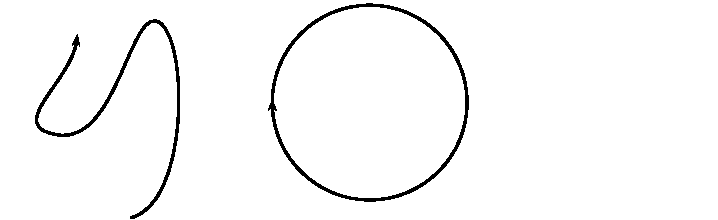
\includegraphics[scale=1.1]{figures/orbita-tipos.pdf}
	\caption{Una órbita arbitraria y un ciclo.}
\end{figure}

\section{Ejemplos Clásicos}

\begin{example}[Péndulo matemático] \label{ej:pendulo}
Supongamos que una masa $m$ se encuentra unida al extremo inferior de una varilla de longitud $l$. Sabemos que el arco $s$ de un círculo de radio $l$ se relaciona con el ángulo central $\theta$ mediante la fórmula $s = l\theta$, de manera que la aceleración angular está dada por

$$ a = \dfrac{d^2s}{dt^2} = l \dfrac{d^\theta}{dt^2}.$$

En ausencia de fuerzas externas o amortiguamiento, la única fuerza que actúa sobre la masa es su peso $mg$, cuya componente tangencial es $-mg\sin\theta$, así que por la segunda ley de Newton:

$$ ml \dfrac{d^2\theta}{dt^2} = ma = -mg\sin\theta.$$

\begin{figure} \label{fig:pendulo} \centering
	\includegraphics[scale=1.35]{figures/pendulum.pdf}
	\caption{Ilustración del péndulo matemático.}
\end{figure}

De donde se deduce la ecuación de segundo orden para $\theta$:

\begin{equation} \label{eq:pendulo0}
	\dfrac{d^2\theta}{dt^2} + \frac{g}{l}\sin\theta = 0.
\end{equation}

Dependiendo de la longitud $l$ de la varilla, la razón $g/l$ cambia, de manera que la ecuación \ref{eq:pendulo0} puede reescribirse como

\begin{equation} \label{eq:pendulo}
	\dfrac{d^2\theta}{dt^2} + \lambda\sin\theta = 0.
\end{equation}

A menudo se asumirá que $\lambda = 1$ al estudiar el péndulo matemático.

Sabemos que la ecuación \ref{eq:pendulo} puede reescribirse como un sistema plano haciendo $x_1 = \theta$ y $x_2 = \dot{\theta}$ obteniendo así:

\begin{equation}
	\begin{array}{l}
		\dot{x_1} = x_2 \\
		\dot{x_2} = -\lambda \sin\theta.
	\end{array}
\end{equation}

Debido a que el término $\sin\theta$ hace que la ecuación anterior sea no lineal, a veces se aproxima, para $\theta$ pequeño, $\sin(\theta) \approx \theta$, obteniéndose en lugar de \ref{eq:pendulo} la ecuación lineal

$$ \ddot{\theta} + \lambda\theta = 0,$$

conocida como oscilador armónico lineal y que ya se estudió en el ejemplo \ref{ex:osciladorarmonico}.


\begin{figure}[!ht] \label{fig:pendulomatematico} \centering
	\includegraphics[scale=0.5]{figures/pendulomatematico-fase.png}
	\caption{Diagrama de fase del péndulo, con centros $(n\pi, 0)$ para $n \in \Z$.}
\end{figure}

\end{example}

\begin{example}[Modelo depredador-presa de Lotka-Volterra]\label{ex:lotkavolterra}

Consideremos dos poblaciones que interactúan entre sí: una especie de presa $x_1$ y su depredador, $x_2$. Un modelo matemático para la población de ambas especies es el modelo \emph{depredador-presa} de Lotka y Volterra, propuesto inicialmente por Alfred J. Lotka \cite{lotka10,lotka25,volterra} y que opera bajo las siguientes suposiciones:

\begin{enumerate}
	\item La población de presa $x_1$ no sufre de escasez de comida ni otros factores ambientales en su contra.
	\item La alimentación de la población depredadora $x_2$ depende exclusivamente del tamaño de la población presa $x_2$.
	\item La tasa de cambio de la población es proporcional a su tamaño.
\end{enumerate}

El sistema Lotka-Volterra corresponde entonces, al par de ecuaciones diferenciales
\begin{equation} \label{eq:lotkavolterra}
	\begin{array}{lll}
		\dot{x_1} & = & a_1x_1 - a_2x_1x_2 \\
		\dot{x_2} & = & -a_3x_2 + a_4x_1x_2,
	\end{array}
\end{equation}

donde $a_1, a_2, a_3$ y $a_4$ son constantes positivas.

Aunque el modelo es simple tiene sentido físico: en ausencia de interacción entre las especies ($a_2 = a_4 = 0$) el modelo se reduce a uno en el que la población presa $x_1$ crece sin límite, mientras que la población de depredadores $x_2$ se extingue eventualmente.
En cambio, cuando hay interacciones (que se consideran proporcionales al producto de las poblaciones $x_1x_2$) el crecimiento de $x_1$ se ve afectado mientras que la tasa de crecimiento de $x_2$ mejora, como es de esperarse.

\begin{figure}
\end{figure}

Es fácil verificar que el sistema \ref{eq:lotkavolterra} tiene dos puntos críticos: a saber $(0,0)$ y $(a_3 / a_4, a_1 / a_2)$.
La estabilidad del primero de ellos puede tratarse mediante linealización (ver sección \ref{sec:linealizacion}) y resulta ser de punto de silla.

Sin embargo, el otro punto crítico es no hiperbólico de manera que debe hacerse un análisis distinto al de linealización. No es difícil concluir, en este caso, que se trata de un centro (ver sección \ref{subsec:centrooespiral}) y que los niveles de la población de presa y depredador oscilan alrededor de este punto fijo.

\begin{figure} \label{fig:lotkavolterra} \centering
	\includegraphics[scale=0.5]{figures/lotkavolterra.png}
	\caption{Diagrama de fase del modelo presa-depredador de Lotka-Volterra.}
\end{figure}

El modelo Lotka-Volterra no tiene en consideración la competencia entre las propias especies ya sea por la obtención de los recursos naturales (en el caso de la presa) o por el número limitado de presas (en el caso de los depredadores). Un sistema más realista que tiene presente estas interacciones se conoce como modelo de \emph{especies en competencia} (ver, por ejemplo, \cite[p.~171]{dynandbif}).

\end{example}

\begin{example}[Oscilador de Van der Pol] \label{ex:vanderpol}

Además de los fenómenos biológicos, el estudio de los circuitos eléctricos también da origen a ecuaciones diferenciales importantes: el \emph{oscilador de Van der Pol} es un tipo de oscilador con amortiguamiento no lineal, planteado por el físico holandés Balthasar Van der Pol \cite{vanderpol} que obedece la ecuación diferencial de segundo orden

\begin{equation} \label{eq:vanderpol}
	\ddot{x} - \lambda (1-x^2)\dot{x} + x = 0.
\end{equation}

Aquí, $x$ es la posición (dependiente de $t$) y $\lambda$ es un parámetro que determina la no linealidad y el amortiguamiento.

La forma bidimensional de la ecuación \ref{eq:vanderpol} corresponde al sistema

\begin{equation} \label{eq:vanderpol2}
	\begin{array}{l}
		\dot{x_1} = x_2 \\
		\dot{x_2} = \lambda (1-x_1^2)x_2 - x_1.
	\end{array}	
\end{equation}

Cuando $\lambda = 0$ la ecuación \ref{eq:vanderpol} se reduce a la del oscilador armónico lineal. En cualquier otro caso ($\lambda > 0$) el sistema \ref{eq:vanderpol2} posee un ciclo límite (ver teorema \ref{teo:poincarebendixson}) y el punto crítico en el origen es inestable.

\begin{figure}[!ht] \label{fig:vanderpol} \centering
	\includegraphics[scale=0.45]{figures/vanderpol.png}
	\caption{Diagrama de fase del oscilador de Van der Pol. Se evidencia el ciclo límite.}
\end{figure}

\end{example}


\chapter{Sistemas Lineales}

Nos concentramos, en este capítulo en sistemas planos $\dot{x} = f(x)$ donde la función $f: \R^2 \to \R^2$ es un mapeo lineal. Es decir, el sistema tiene la forma:

\begin{equation} \label{eq:sistemalineal}
	\begin{array}{l}
		\dot{x_1} = a_{11}x_1 + a_{12}x_2 \\
		\dot{x_2} = a_{21}x_1 + a_{22}x_2,
	\end{array}
\end{equation}

donde cada $a_{ij} \in \R$.

Si hacemos

$$ A = \left(
\begin{array}{ll}
	a_{11} & a_{12} \\
	a_{21} & a_{22}
\end{array}
\right),
$$

podemos reescribir el sistema \ref{eq:sistemalineal} en la forma vectorial equivalente

\begin{equation} \label{eq:sistemalinealv}
	\dot{x} = f(x) = Ax.
\end{equation}

Podemos anticipar desde ya que hay un punto crítico del sistema en $\bar{x} = 0$.

\section{Propiedades de las soluciones}

A continuación hacemos un repaso de algunos resultados importantes acerca de las soluciones de sistemas lineales planos autónomos. Las pruebas de los resultados se pueden encontrar en cualquier texto elemental de ecuaciones diferenciales, como podrían ser \cite{zillcull} o \cite{boycediprima}.

\theorem{Todo solución $X$ de un sistema lineal plano tiene la forma $$ x = c_1u+ c_2v, $$ donde $u, v$ son soluciones linealmente independientes de \ref{eq:sistemalinealv} y $c_1, c_2$ son constantes.}

En vista del teorema anterior, el problema se reduce a encontrar dos soluciones $u, v$ que sean linealmente independientes. Tal conjunto de soluciones se conoce como \emph{conjunto fundamental de soluciones} y a $x = c_1u + c_2v$ se le conoce como \textit{solución general}.

Las constantes $c_1$ y $c_2$ quedan determinadas una vez se especifica la condición inicial $x(0) = x^0$.

\begin{lemma}[Criterio para la independencia lineal de soluciones]
Dos soluciones $u$ y $v$ del sistema \ref{eq:sistemalinealv} definidas sobre un intervalo $I$ son linealmente independientes si y sólo si el determinante \emph{wronskiano}

$$ W(u,v)(t) = \left|
	\begin{array}{ll}
		u_1(t) & v_1(t) \\
		u_2(t) & v_2(t)
	\end{array}
\right|$$

es no nulo para toda $t \in I$.
\end{lemma}

\begin{example}
Consideremos el sistema plano

$$
	\begin{array}{l}
		\dot{x_1} = x_1 + 3x_2 \\
		\dot{x_2} = 5x_1 + 3x_2
	\end{array},
$$

que tiene forma vectorial

$$ \dot{x} = \left(
	\begin{array}{ll}
		1 & 3 \\ 5 & 3
	\end{array}
\right) x.$$

Es fácil verificar que las funciones $u(t) = (e^{-2t}, -e^{-2t})$ y $v(t) = (3e^{6t}, 5e^{6t})$ son soluciones del sistema.

Más aún, estas soluciones son linealmente independientes y forman un conjunto fundamental de soluciones pues

$$
	W(u,v)(t) =
\left|
	\begin{array}{ll}
		e^{-2t} & 3e^{6t} \\
		-e^{-2t} & 5e^{6t}
	\end{array}
\right| = 5e^{4t} + 3e^{4t} = 8e^{4t} \neq 0,
$$

para todo $t \in \R$.

Esto significa que toda solución del sistema tiene la forma

$$ x(t) = \left( \begin{array}{l} x_1(t) \\ x_2(t) \end{array} \right)
= c_1 \left( \begin{array}{l} e^{-2t} \\ -e^{-2t} \end{array} \right) + c_2 \left( \begin{array}{l} 3e^{6t} \\ 5e^{6t} \end{array} \right).$$
\end{example}

Por analogía a la teoría de ecuaciones diferenciales lineales de primer orden (ver, por ejemplo, \cite{zillcull,boycediprima}), buscamos soluciones del sistema \ref{eq:sistemalinealv} que tengan la forma
\begin{equation} \label{eq:solexponencial}
x(t) = (k_1e^{\lambda t}, k_2e^{\lambda t}).
\end{equation}

Supongamos que $x$ es una solución forma \ref{eq:solexponencial}. Entonces

$$ \dot{x} = (k_1 \lambda e^{\lambda t}, k_2 \lambda e^{\lambda t}). $$

Si reemplazamos $x$ y $\dot{x}$ en la ecuación $\dot{x} = f(x) = Ax$ y hacemos $K = (k_1, k_2)$ obtenemos

$$
	K \lambda e^{\lambda t} = A (Ke^{\lambda t}).
$$

Como $e^{\lambda t} \neq 0$ podemos dividir ambos lados de la ecuación anterior por $e^{\lambda t}$ y reordenando se obtiene

$$ AK = \lambda K$$

o equivalentemente

\begin{equation} \label{eq:ecvalorpropio}
	(A - \lambda I) K = 0.
\end{equation}

Lo anterior significa que si $x = x(t)$ es una solución de la forma propuesta, entonces $\lambda$ y $K$ deben satisfacer \ref{eq:ecvalorpropio}. Es decir, $\lambda$ debe ser un valor propio de $A$ y $K$ un vector propio asociado a este valor propio $\lambda$.

En estas condiciones, $$ x = K e^{\lambda t}$$ es siempre solución de $\dot{x} = Ax$.

El resto de esta sección está dedicado a la obtención de dos soluciones que sean linealmente independientes $u$ y $v$ de manera que podamos escribir siempre la solución general de la forma antes descrita en términos de estas dos soluciones.

En virtud de lo anterior es lógico que las soluciones dependan de la forma de los valores propios de $A$: como $\det(A - \lambda I) = 0$ es una ecuación algebraica de segundo grado, estos pueden ser reales y distintos, reales repetidos o complejos conjugados.

\subsection{Ecuación Característica}

Para hallar los valores propios $\lambda$ de la matriz $A$ 2x2 del sistema \ref{eq:sistemalinealv} computamos las raíces de la ecuación característica $\det(A - \lambda I) = 0$.

Notamos que
\begin{eqnarray*}
	\det(A - \lambda I) & = &  \left| \begin{array}{ll} a_{11} - \lambda & a_{12} \\ a_{21} & a_{22} - \lambda \end{array} \right| \\ 
	& = & (a_{11} - \lambda)(a_{22} - \lambda) - a_{12}a_{21} \\
	& = & \lambda^2 - (a_{11} + a_{22})\lambda + (a_{11}a_{22} - a_{12}a_{21}).
\end{eqnarray*}

Si escribimos $\Delta = \det(A) = a_{11}a_{22} - a_{12}a_{21}$ y $\tau = a_{11} + a_{22}$, la traza de $A$, entonces la ecuación característica es:

\begin{equation} \label{eq:eccaracteristica}
	\lambda^2 - \tau \lambda + \Delta = 0.
\end{equation}

Por lo tanto los valores propios de $A$ son $\lambda_{1,2} = (\tau \pm \sqrt{\tau^2 - 4\Delta}) / 2 $ que pueden ser reales distintos, reales repetidos y complejos conjugados según $\tau^2 - 4\Delta$ sea positivo, cero o negativo.

\subsection{Solución General} \label{subsec:soluciongeneral}

Enunciamos, sin prueba, un teorema acerca de la solución general del sistema para cada uno de estos casos.

\begin{theorem}[Solución para valores propios reales distintos]Si $\tau^2 - 4\Delta > 0$ entonces la ecuación característica \ref{eq:eccaracteristica} tiene dos raíces reales $\lambda_1$ y $\lambda_2$ distintas y la solución general del sistema lineal plano $\dot{x} = Ax$ está dada por

\begin{equation} \label{eq:solvlrspropiosdistintos}
x = x(t) = c_1(K_1 e^{\lambda_1 t}) + c_2(K_2 e^{\lambda_2 t}),
\end{equation}

donde $K_1$ es un vector propio asociado al valor propio $\lambda_1$ y $K_2$ uno asociado al valor propio $\lambda_2$.
\end{theorem}

\begin{theorem}[Solución para valores propios reales repetidos]Si $\tau^2 - 4\Delta = 0$ entonces la ecuación característica \ref{eq:eccaracteristica} tiene una raíz real $\lambda_1$ de multiplicidad dos.

\begin{itemize}

\item Si existen dos vectores propios linealmente independientes $K_1, K_2$ asociados a $\lambda_1$ entonces la solución general del sistema lineal plano $\dot{x} = Ax$ está dada por

\begin{equation} \label{eq:solvlrspropiosrepetidos1}
x = x(t) = c_1(K_1 e^{\lambda_1 t}) + c_2(K_2 e^{\lambda_1 t}).
\end{equation}

\item Si sólo se tiene un vector propio linealmente independiente $K_1$ entonces la solución general del sistema lineal plano $\dot{x} = Ax$ tiene la forma

\begin{equation} \label{eq:solvlrspropiosrepetidos2}
x = x(t) = c_1(K_1 e^{\lambda_1 t}) + c_2(K_1 t e^{\lambda_1 t} + Pe^{\lambda_1 t}),
\end{equation}

donde $P$ es un vector tal que $(A-\lambda_1I)P=K_1$.
\end{itemize}

\end{theorem}


\begin{theorem}[Solución para valores propios complejos conjugados]Si $\tau^2 - 4\Delta < 0$ entonces la ecuación característica \ref{eq:eccaracteristica} tiene dos raíces complejas conjugadas $\lambda_{1,2} = a \pm i b$ y la solución general del sistema lineal plano $\dot{x} = Ax$ está dada por

\begin{equation} \label{eq:solvlrspropioscomplejos}
x = x(t) = c_1 e^{a t}(B_1 \cos(bt) - B_2 \sin(bt)) + c_2 e^{a t}(B_2 \cos(bt) + B_1 \sin(bt)),
\end{equation}

donde $K_1 = B_1 + iB_2$ es un vector propio asociado al valor propio $\lambda_1$.
\end{theorem}

\section{Clasificación y estabilidad de puntos críticos ($\Delta \neq 0$)} \label{sec:estabilidadlineal}

Si $A$ es no singular ($\det(A) = \Delta \neq 0$), el único punto crítico del sistema lineal plano $\dot{x} = f(x) = Ax$ es $\bar{x} = 0$.

El comportamiento cualitativo de las soluciones que no son de equilibrio, en un sistema lineal, es muy similar y nos permite establecer una clasificación para el punto crítico $\bar{x} = 0$.

Hemos visto ya en ejemplos anteriores que algunas soluciones se alejan o acercan a los puntos críticos, otras se enrollan alrededor del punto crítico, etc. A continuación justificaremos cada uno de estos posibles casos según sean los valores propios de $A$ (como se vio en la sección anterior).

\subsection{Valores propios reales distintos y negativos (nodo estable)}
Consideramos el caso $\tau^2 - 4\Delta > 0$ y $\lambda_1, \lambda_2$ son valores propios de $A$ tales que $\lambda_1 < 0, \lambda_2 < 0$.

En este caso, toda solución es de la forma \ref{eq:solvlrspropiosdistintos}:

$$ x = c_1(K_1 e^{\lambda_1 t}) + c_2(K_2 e^{\lambda_2 t}). $$

Podemos reescribir la solución como

$$ x = e^{\lambda_1 t} [ c_1 K_1 + c_2K_2 e^{(\lambda_2 - \lambda_1)t} ].$$

Supongamos sin pérdida de generalidad que $\lambda_2 < \lambda_1 < 0$, entonces de acuerdo a la ecuación anterior $x(t) \to 0$ cuando $t \to \infty$.
A largo plazo, $x(t) \approx c_1K_1e^{\lambda_1 t}$ y por lo tanto si $c_1 \neq 0$ entonces $x \to 0$ a lo largo de la recta determinada por el vector propio $K_1$.
Si en cambio, $c_1 = 0$ entonces $x(t) = c_2 K_2 e^{\lambda_2 t}$ y $x \to 0$ desde una de las direcciones determinadas por el vector propio $K_2$.

En particular si el punto inicial $x^0$ está en alguna de las rectas determinadas por $K_1$ o $K_2$ la solución tiende a 0 a través de la recta.

En cualquier caso, $x \to 0$ y decimos que el punto crítico $\bar{x} = 0$ es un \emph{nodo (estable)} o \emph{sumidero nodal}.

\subsection{Valores propios reales distintos y positivos (nodo inestable)}

Como antes, $\tau^2 - 4\Delta > 0$ pero ahora $\lambda_1 > 0$ y $\lambda_2 > 0$.
Toda solución solución puede escribirse también como

$$ x = e^{\lambda_1 t} [ c_1 K_1 + c_2K_2 e^{(\lambda_2 - \lambda_1)t} ].$$

Supondremos, de nuevo, que $\lambda_1 > \lambda_2$. Entonces a largo plazo $|x(t)| \approx |c_1 K_1 e^{\lambda_1 t}| \to \infty$ cuando $t \to \infty$.

El patrón de las trayectorias es idéntico al caso anterior pero estas se alejan del punto crítico $\bar{x} = 0$ en lugar de acercarse. En este caso el punto crítico $\bar{x} = 0$ se llama \emph{nodo (inestable)} o \emph{sumidero nodal}.

\begin{figure}[!ht] \label{fig:nodos} \centering
    \includegraphics[scale=1.0]{figures/nodoestable.pdf}\\(a)\\
    \includegraphics[scale=1.0]{figures/nodoinestable.pdf}\\(b)\\
    \includegraphics[scale=1.0]{figures/puntodesilla.pdf}\\(c)\\
    \caption{(a) Nodo estable, (b) Nodo inestable, (c) Punto de silla.}
\end{figure}

\subsection{Valores propios reales distintos y de signo opuesto (punto de silla)}

De nuevo la solución es de la forma

$$ x = c_1(K_1 e^{\lambda_1 t}) + c_2(K_2 e^{\lambda_2 t}). $$

Suponemos que $\lambda_2 < \lambda_1$.

Si $c_1 = 0$ (por ejemplo, cuando $x^0$ está sobre la recta determinada por $K_2$) entonces como $\lambda_2 < 0$, $x \to 0$ a lo largo de esta recta.
Si $c_2 = 0$ (por ejemplo, cuando $x^0$ está sobre la recta determinada por $K_1$) entonces dado que $\lambda_1 >0$, $||x|| \to \infty$ a lo largo de la recta determinada por $K_1$.

Las soluciones que parten de otros puntos iniciales, para las cuales $c_1 \neq 0$ y $c_2 \neq 0$ el término dominante en la solución es $e^{\lambda_1 t}$ y como $\lambda_1 > 0$ entonces las soluciones se hacen no acotadas a medida que aumenta $t$ de manera asintótica a la recta determinada por $K_1$.

Resumiendo, las soluciones que no comienzan en ninguna de las rectas determinadas por $K_1$ o $K_2$ son tales que $||x|| \to \infty$ y lo hacen de manera asintótica a la recta determinada por $K_1$. De otro lado, las únicas soluciones que tienden al punto de equilibrio $\bar{x} = 0$ son aquellas que comienzan sobre la recta determinada por $K_2$ y lo a lo largo de dicha recta.

En este caso, el punto crítico se llama \emph{punto de silla} y es, evidentemente, un equilibrio inestable.

\subsection{Valor propio real repetido (nodo degenerado)}

En este caso $\tau^2 - 4\Delta = 0$ y hay un único valor propio real de multiplicidad dos: $\lambda_{1,2} = \lambda$.

\subsubsection{Dos vectores propios linealmente independientes (nodo propio degenerado)}

Si se pueden conseguir dos vectores propios $K_1$ y $K_2$ linealmente independientes asociados al valor propio $\lambda$ entonces toda solución es de la forma \ref{eq:solvlrspropiosrepetidos1}, que puede reescribirse como
$$ x = (c_1K_1 + c_2K_2)e^{\lambda t}.$$

En este caso el punto crítico $\bar{x} = 0$ se dice \emph{nodo propio}, \emph{nodo degenerado} o \emph{punto estrella} y es estable o inestable según $\lambda < 0$ o $\lambda > 0$ respectivamente.

\begin{figure}[!ht] \label{fig:nodopropio} \centering
    \includegraphics[scale=1.0]{figures/nodopropio.pdf}
    \caption{Nodo propio degenerado.}
\end{figure}

\subsubsection{Un solo vector linealmente independiente (nodo impropio degenerado)}

En este caso apenas es posible conseguir un vector propio $K_1$ linealmente independiente asociado al valor propio $\lambda$. Las soluciones, según la fórmula \ref{eq:solvlrspropiosrepetidos2}, son de la forma:
$$ x =c_1(K_1 e^{\lambda t}) + c_2(K_1 t e^{\lambda t} + Pe^{\lambda t}). $$

El comportamiento de todas las soluciones $x = x(t)$ es similar: la recta determinada por $K_1$ es una asíntota y $||x|| \to 0$ si $\lambda < 0$ o $||x|| \to \infty$ si $\lambda > 0$.

Si $\lambda < 0$ entonces el punto crítico $\bar{x} = 0$ se llama \emph{nodo impropio estable} o simplemente \emph{nodo degenerado estable} y si $\lambda > 0$ el punto crítico $\bar{x} = 0$ se llama \emph{nodo impropio inestable} o \emph{nodo generado inestable}.

\begin{figure}[!ht] \label{fig:nodoimpropio} \centering
    \includegraphics[scale=1.0]{figures/nodoimpropio.pdf}
    \caption{Nodo impropio degenerado.}
\end{figure}

\subsection{Valores propios complejos conjugados (centro, punto de espiral)} \label{subsec:centrooespiral}

Finalmente, estamos en el caso en el que $\tau^2 - 4\Delta < 0$ y los valores propios de $A$ son complejos conjugados: $\lambda_{1,2} = a \pm ib$.

Si $K_1 = B_1 + iB_2$ es un vector propio asociado al valor propio $\lambda_1 = a + ib$ entonces, por la fórmula \ref{eq:solvlrspropioscomplejos} la solución es de la forma

$$ x = c_1 e^{a t}(B_1 \cos(bt) - B_2 \sin(bt)) + c_2 e^{a t}(B_2 \cos(bt) + B_1 \sin(bt)).$$

\subsubsection{Valor propio imaginario puro}
Cuando $\tau = 0$, $\lambda_1$ es un imaginario puro y la solución se puede escribir como

$$ x = C_1 \cos(bt) + C_2 \sin(bt), $$

donde $C_1$ y $C_2$ son vectores constantes. Esto implica que todas las soluciones son periódicas con período $2\pi / b$ y es fácil ver que corresponden a elipses centradas en el origen.

En este caso el punto crítico $\bar{x} = 0$ se llama \emph{centro} y la orientación de todas las órbitas es la misma.

\subsubsection{Valor propio con parte real no nula}

Si $\tau \neq 0$ entonces los valores propios tienen parte real $a \neq 0$ y las órbitas del sistema son espirales que se alejan o acercan todas al punto crítico $\bar{x} = 0$ debido al término $e^{a t}$ que aparece en la solución.

El punto crítico se llama un \emph{punto espiral} y es estable cuando $\lambda < 0$ e inestable cuando $\lambda > 0$.

Cuando el punto espiral es estable se le llama también \emph{sumidero espiral} y cuando es inestable \emph{fuente espiral}.

\begin{figure}[!ht] \label{fig:centroyespiral} \centering
    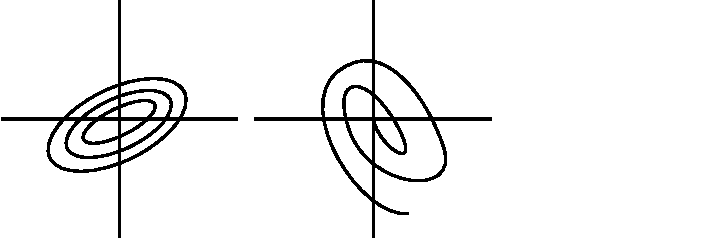
\includegraphics[scale=1.0]{figures/centroyespiral.pdf}  
    \caption{Centro y punto de espiral.}
\end{figure}

\section{Clasificación y estabilidad de puntos críticos ($\Delta = 0$)}

Cuando el sistema plano es $\dot{x} = f(x) = Ax$ con $A$ una matriz singular (i.e. $\det(A) = \Delta = 0$) entonces es un resultado elemental del álgebra lineal que hay una infinidad de puntos críticos (soluciones a $Ax = 0$) además del origen $x = 0$.

Las soluciones en la sección \ref{subsec:soluciongeneral} siguen siendo válidas en este caso, aunque se advierte ya de la ecuación característica \ref{eq:eccaracteristica} que los valores propios son $\lambda_1 = 0$ y $\lambda_2 \in \R$.

Consideramos a continuación varios casos.

\subsection{A es la matriz cero ($A = 0$)}
En este caso todo punto $x \in \R^2$ es un punto crítico, así que toda trayectoria en el plano de fase es trivial.

\begin{figure}[!ht] \centering
    \includegraphics[scale=1.0]{figures/amatriz0.pdf}  
\end{figure}


\subsection{$\lambda_1 = 0, \lambda_2 < 0$}
Es posible demostrar que en este caso el sistema es topológicamente equivalente (ver \cite[p.~239]{dynandbif}) a uno con matriz de coeficientes

$$ A = \left( \begin{array}{ll} -1 & 0 \\ 0 & 0 \end{array} \right).$$

Por lo tanto, el diagrama de fase es similar a la figura siguiente, donde todo punto $(0,x_2)$ es de equilibrio.

\begin{figure}[!ht] \centering
    \includegraphics[scale=1.0]{figures/asingular_1.pdf}
\end{figure}

\subsection{$\lambda_1 = 0, \lambda_2 > 0$}
De nuevo, como en \cite[p.~239]{dynandbif}, es posible verificar que este sistema es topológicamente equivalente a uno con matriz de coeficientes

$$ A = \left( \begin{array}{ll} 1 & 0 \\ 0 & 0 \end{array} \right).$$

Por lo tanto, el diagrama de fase es similar a la figura siguiente, donde todo punto $(0,x_2)$ es de equilibrio pero el sentido de las flechas es contrario al del caso anterior.

\begin{figure}[!ht] \centering
    \includegraphics[scale=1.0]{figures/asingular1.pdf}
\end{figure}

\subsection{$\lambda_1 = \lambda_2 = 0$}
En este caso tanto $\Delta$ como $\tau$ son nulos. Esto es, $a_{11}a_{22} - a_{12}a_{21} = 0$ y también $a_{11} + a_{22} = 0$.
Es posible analizar el comportamiento de las soluciones y puntos de equilibrio a partir de estas ecuaciones considerando los distintos casos $a_{11} = 0$ o $a_{11} \neq 0$, etc.

Sin embargo, cualquiera sea el caso el sistema es equivalente (ver \cite[teorema 8.16 p.~239]{dynandbif}) a uno con matriz de coeficientes

$$ A = \left( \begin{array}{ll} 0 & 1 \\ 0 & 0 \end{array} \right),$$

cuyo diagrama de fase aparece es como a continuación.

\begin{figure}[!ht] \centering
    \includegraphics[scale=1.0]{figures/asingularr1.pdf}
\end{figure}

\begin{remark}Aunque no se dijo explícitamente para cada caso, es claro que todos los puntos de equilibrio son \emph{inestables} si $\Delta = 0$.
\end{remark}

\section{Criterio de estabilidad para sistemas lineales}
Resumimos los resultados de las dos secciones previas:

\begin{theorem}[Criterio de estabilidad para sistemas lineales] \label{teo:criterioestabilidadlineales}
Sea $\dot{x} = f(x) = Ax$ un sistema plano lineal y $\bar{x}$ un punto de equilibrio del mismo.

\begin{enumerate}[(a)]
	\item Si $\det(A) \neq 0$ y todos los valores propios de $A$ tienen parte real negativa o son imaginarios puros, $\bar{x} = 0$ es un punto crítico asintóticamente estable (y por tanto estable).
	\item Si $\det(A) = 0$ o hay valores propios de $A$ con parte real positiva, el punto crítico $\bar{x}$ es inestable.
\end{enumerate}

Debido a lo anterior a menudo la clasificación de puntos críticos y estabilidad se realiza según los valores propios de $A$ tenga o no parte real no nula.

\begin{definition}[Matriz hiperbólica] Decimos que $A$ es \emph{hiperbólica} si todos sus valores propios tienen parte real no nula.
\end{definition}

Con esta definición, notamos que la estabilidad de un punto de equilibrio de un sistema lineal con matriz de coeficientes hiperbólica depende exclusivamente del signo de la parte real.

\end{theorem}

\chapter{Sistemas No Lineales}
Consideramos en este capítulo sistemas planos autónomos $\dot{x} = f(x)$ donde $f$ es una función no necesariamente lineal en $x = (x_1,x_2)$.

Supondremos $f$ de al menos clase $C^1$ de manera que sea posible considerar la linealización de $f$ mediante su derivada (matriz jacobiana) y estudiar las propiedades de este sistema lineal con el objetivo de deducir información sobre el comportamiento del sistema original.

A continuación formalizamos el concepto de linealización mediante expansión en serie de Taylor (sección \ref{sec:linealizacion}).

\section{Linealización} \label{sec:linealizacion}

Consideremos un sistema plano como en la ecuación \ref{eq:sistema_dinamico_plano_v0}, de la forma

\begin{equation}
	\dot{x} = f(x) = (f_1(x_1,x_2), f_2(x_1,x_2)),
\end{equation}

donde $f$ es una función arbitraria de clase $C^1$.

En este caso no necesariamente el sistema tiene un punto crítico en $x = 0$ y mucho menos debe ser el único.

\begin{example}Como vimos en el ejemplo \ref{ej:pendulo}, el péndulo matemático está descrito por la ecuación diferencial de segundo orden $\ddot{x} + \sin(x) = 0$ que puede escribirse en forma vectorial con $x = (x_1,x_2)$ como

$$
\begin{array}{lll}
	\dot{x_1} & = & x_2 \\
	\dot{x_2} & = & -\sin(x_1).
\end{array}
$$

Por lo tanto el péndulo matemático tiene un punto crítico en $(x_1,x_2) = (0,0)$ pero también en todos los puntos $(n\pi, 0)$ para $n \in \Z$.
\end{example}

Supongamos entonces que $x^1, x^2, ..., x^n, ...$ son puntos críticos del sistema $\dot{x} = f(x)$ y que son aislados (es decir, existe una vecindad  $V_i$ de $x^i$ donde $x^i$ es el único punto crítico).

Sea $\bar{x}$ uno de estos puntos críticos y supongamos que $f$ es diferenciable en $\bar{x}$. Entonces podemos expandir $f$ como serie de Taylor alrededor de $f$ y escribir para $x$ cerca de $\bar{x}$:

\begin{equation} \label{eq:expansiontaylor1}
	f(x) = f(\bar{x}) + Df(\bar{x})(x - \bar{x}) + h(x)
\end{equation}

donde $|| \frac{h(x)}{x - \bar{x}}|| \to 0$ cuando $x \to \bar{x}$.

Ahora, como $\bar{x}$ es un punto crítico entonces $f(\bar{x}) = 0$ y la fórmula \ref{eq:expansiontaylor1} se reduce a 

\begin{equation}
	f(x) = Df(\bar{x})(x - \bar{x}) + h(x).
\end{equation}

Por lo tanto, el sistema no lineal, cerca de $\bar{x}$ es

$$ \dot{x} = f(x) = Df(\bar{x})(x - \bar{x}) + h(x).$$

Si a continuación introducimos el cambio de coordenadas $y = x - \bar{x}$ entonces tenemos 

\begin{equation} \label{eq:cuasilineal}
	\dot{y} = Df(\bar{x})y + g(y).
\end{equation}

En la ecuación \ref{eq:cuasilineal}, $g(0) = 0$ y $Dg(0) = 0$ así que el Teorema del Valor Medio implica que $g(y)$ es ``pequeño'' en comparación a $y$ cerca del origen. Más precisamente, dado $m > 0$ existe $\delta > 0$ tal que 

$$ ||g(y)|| \leq m||y||$$

siempre que $||y|| < \delta$.

En otras palabras, $g(y)$ puede hacerse tan pequeño como se desee tomando $y$ suficientemente pequeño. Por esta razón resulta natural pensar que la estabilidad de $\bar{x}$ pueda describirse en términos del sistema lineal

\begin{equation} \label{eq:linealizacion}
	\dot{y} = Df(\bar{x})y.
\end{equation}

Si $Df(\bar{x})$ es invertible, el único punto crítico es $\bar{y} = 0$ y puede clasificarse según los criterios vistos en la sección \ref{sec:estabilidadlineal}.
Se quisiera poder llegar a las mismas conclusiones para $\bar{x}$, pero esto no será siempre posible como se verá más adelante.

\section{Criterio de estabilidad para sistemas no lineales}
A partir de la linealización de $f$ en un punto crítico $\bar{x}$ es posible a veces determinar la estabilidad del mismo de manera análoga al caso lineal (teorema \ref{teo:criterioestabilidadlineales}).

El siguiente teorema, cuya prueba puede encontrarse en \cite[p.~267,272]{dynandbif}, describe la estabilidad en dos casos particulares.

\begin{theorem}[Criterio de estabilidad para sistemas no lineales] \label{teo:criterioestabilidadnolineales}
Sea $f$ de clase $C^1$, $\dot{x} = f(x)$ un sistema plano y $\bar{x}$ un punto crítico del mismo.

\begin{enumerate}[(a)]
	\item Si todos los valores propios de $Df(\bar{x})$ tienen parte real negativa, entonces $\bar{x}$ es un punto crítico asintóticamente estable (y por lo tanto, estable).
	\item Si al menos un valor propio de $Df(\bar{x})$ tiene parte real positiva entones $\bar{x}$ es un punto crítico inestable.
\end{enumerate}
\end{theorem}

\begin{example} \label{ex:nolinealhiperbolico}
Considérese el sistema no lineal

$$ \begin{array}{l} \dot{x_1} = x_1^2 + x_2^2 - 6 \\ \dot{x_2} = x_1^2 - x_2 \end{array}. $$

Los puntos críticos son $(\sqrt{2}, 2)$ y $(-\sqrt{2}, 2)$ y la matriz jacobiana $Df(x)$ está dada por

$$ Df(x) = \left( \begin{array}{ll} 2x_1 & 2x_2 \\ 2x_1 & -1 \end{array} \right).$$

Sean

$$
	A_1 = Df((\sqrt{2},2)) = \left(\begin{array}{ll} 2\sqrt{2} & 4 \\ 2\sqrt{2} & -1 \end{array} \right), \hspace{8pt}
	A_2 = Df((-\sqrt{2},2)) = \left(\begin{array}{ll} -2\sqrt{2} & 4 \\ -2\sqrt{2} & -1 \end{array} \right).	
$$

$A_1$ tiene un valor propio real positivo pues $\det(A_1) < 0$ así que puede concluirse que $(\sqrt{2}, 2)$ es un punto crítico inestable.
Por otro lado, $A_2$ tiene determinante positivo y traza negativa, así que ambos valores propios tienen partes reales negativas. Por el criterio de estabilidad, $(-\sqrt{2},2)$ es un punto crítico estable.

Aunque aún no podemos asegurarlo (más adelante se hará) podríamos pensar que el punto crítico $(-\sqrt{2}, 2)$ es un punto de espiral. Este sería el caso si el sistema fuera lineal y, como ilustra la figura \ref{fig:nolinealhiperbolico-espiral}, la evidencia numérica refuerza esta idea.

\begin{figure} \label{fig:nolinealhiperbolico-espiral} \centering
\includegraphics[scale=0.45]{figures/nolinealhiperbolico-espiral.png}
\caption{Diagrama de fase en cercanías del punto crítico $(-\sqrt{2}, 2)$.}
\end{figure}

\end{example}

Nótese que el teorema \ref{teo:criterioestabilidadnolineales} no ofrece información alguna para cuando hay valores propios con parte real nula. Esto no es casualidad pues en tal caso no es posible determinar la naturaleza del punto crítico a partir de la linealización, como ilustra el siguiente ejemplo.

\begin{example} \label{ex:nolinealnohiperbolico}
Sea $\mu \in \R$ arbitrario y consideremos el sistema no lineal

$$
	\begin{array}{l}
		\dot{x_1} = x_2 + \mu x_1(x_1^2 + x_2^2) \\
		\dot{x_2} = x_1 + \mu x_2(x_1^2 + x_2^2).
	\end{array}
$$

La linealizacíon del sistema en el punto crítico $\bar{x} = 0$ es $\dot{x} = Df(\bar{x})x = \left( \begin{array}{ll} 0 & 1 \\ -1 & 0 \end{array} \right) x,$ sin importar el valor de $\mu$.
Los valores propios de $Df(\bar{x})$ son $\lambda_{1,2} = \pm i$, de manera que no podemos utilizar el criterio de estabilidad pues tienen parte real nula. La razón la ofrece el siguiente argumento.

Notemos que

$$ \dfrac{d}{dt} (x_1^2 + x_2^2) = 2\mu(x_1^2 + x_2^2)^2. $$

Entonces, si $\mu < 0$, $||x(t)|| \to 0$ cuando $t \to \infty$ y por lo tanto $\bar{x} = 0$ es asintóticamente estable.
Si en cambio $\mu > 0$ entonces $||x(t)|| \to \infty$ cuando $t \to \infty$ y el punto crítico $\bar{x} = 0$ resulta ser inestable.

Esta dependencia de $\mu$ no aparece en la linealización del sistema y por lo tanto este ejemplo demuestra que el teorema \ref{teo:criterioestabilidadnolineales} es tan preciso como es posible.
\end{example}


\section{Clasificación de puntos críticos}

Quisiéramos repetir la clasificación hecha en la sección \ref{sec:estabilidadlineal} para los puntos críticos de sistemas no lineales y nombrar los puntos críticos como nodos, puntos de silla, centros, etc.

Por supuesto, la idea es utilizar la linealización para tal fin, sin que sea necesario resolver el sistema de manera explícita.

Desde el principio sabemos que esta tarea no es tan sencilla como en el caso lineal: el ejemplo \ref{ex:nolinealnohiperbolico} demuestra que cuando hay valores propios con parte real nula no podemos ni siquiera determinar utilizando solo la matriz jacobiana la estabilidad del punto crítico, mucho menos deducir si se trata de un centro, punto espiral, nodo, etc.

Por el contrario, si se vuelve al diagrama de fase del ejemplo \ref{ex:nolinealhiperbolico} notamos que no sólo pudimos deducir, utilizando el criterio de estabilidad, la estabilidad de los puntos críticos sino que estos coinciden, además con el tipo de punto crítico del sistema linealizado. Por ejemplo, para $\bar{x} = (-\sqrt{2},2)$ el sistema lineal tiene un punto de espiral y este es el mismo comportamiento que presenta el punto crítico en el sistema no lineal.

Podría pensarse, entonces, que las dificultades aparecen únicamente cuando la matriz jacobiana $Df(\bar{x})$ no es hiperbólica, es decir, tiene valores propios con parte real nula y que, en caso contrario, las soluciones del sistema no lineal tienen el mismo comportamiento geométrico que las del sistema lineal correspondiente. En efecto, este es el caso, como se verá a continuación.

\subsection{Puntos críticos hiperbólicos}

\begin{definition}Un punto crítico $\bar{x}$ de un sistema plano $\dot{x} = f(x)$ es \emph{hiperbólico} si la matriz jacobiana en ese punto, $Df(\bar{x})$ es hiperbólica (tiene valores propios todos con parte real no nula).
\end{definition}

Ya sabemos del ejemplo \ref{ex:nolinealnohiperbolico} que en puntos críticos no hiperbólicos puede ser imposible conocer el comportamiento de las soluciones en vecindad del mismo a partir de la linealización. El caso es contrario cuando se trata de puntos hiperbólicos, como demuestra el siguiente teorema.

\begin{theorem}[Hartman-Grobman] \label{teo:hartmangrobman}
Sea $f$ de clase $C^1$ y $\bar{x}$ un punto crítico \emph{hiperbólico} del sistema plano $\dot{x} = f(x)$. Entonces hay una vecindad de $\bar{x}$ en la cual $\dot{x} = f(x)$ es topológicamente equivalente a su linealización $\dot{x} = Df(\bar{x})x$.
\begin{proof}
Ver \cite[p.~136]{barrvalls}.
\end{proof}
\end{theorem}

El teorema anterior garantiza, entonces, que para puntos críticos hiperbólicos el comportamiento del sistema no lineal cerca del punto es ``idéntico'' al del sistema lineal correspondiente y por tanto todas las nociones antes vistan coinciden.

Para puntos críticos no hiperbólicos es necesario utilizar otras técnicas (o hallar las soluciones del sistema) para determinar el comportamiento.

Combinando el teorema \ref{teo:hartmangrobman} con el criterio de estabilidad (teorema \ref{teo:criterioestabilidadnolineales}) es posible construir la tabla \ref{tab:clasificacionequilibrios}, que clasifica los equilibrios de sistemas no lineales (por supuesto, también aplica para lineales).

\begin{table}[ht!]
	\begin{tabular}{|c|c|c|c|c|}
		\hline
		\textbf{Vlrs propios de $Df(\bar{x})$} & \multicolumn{2}{|c|}{\textbf{Linealización}} & \multicolumn{2}{|c|}{\textbf{Sistema no lineal}} \\
		\hline
		 & \textbf{Tipo} &\textbf{Estabilidad} & \textbf{Tipo} & \textbf{Estabilidad} \\
		\hline
		\multicolumn{5}{|c|}{\textit{Equilibrios Hiperbólicos}} \\
		\hline
		$\lambda_1 > \lambda_2 > 0$ & nodo & inestable & nodo & inestable \\
		$\lambda_1 < \lambda_2 < 0$ & nodo & A. E. & nodo & A. E. \\
		$\lambda_2 < 0 < \lambda_1$ & punto silla & inestable & punto silla & inestable \\
		$\lambda_{1,2} = a \pm ib, a > 0$ & punto espiral & inestable & punto espiral & inestable \\
		$\lambda_{1,2} = a \pm ib, a < 0$ & punto espiral & A. E. & punto espiral & A. E. \\

		\hline
		\multicolumn{5}{|c|}{\textit{Equilibrios no Hiperbólicos}} \\
		\hline
		$\lambda_1 = \lambda_2 >0$ & nodo propio o impropio & inestable & nodo o punto espiral & inestable \\
		$\lambda_1 = \lambda_2 < 0$ & nodo propio o impropio & A. E. & nodo o punto espiral & A. E. \\
		$\lambda_{1,2} = \pm ib$ & centro & estable & centro o punto espiral & \textbf{?} \\
		\hline
	\end{tabular}
	\label{tab:clasificacionequilibrios}
	\caption{Clasificación de equilibrios en sistemas no lineales.}
\end{table}

\chapter{Teorema de Poincaré-Bendixson}

\section{Conjuntos límite y nociones básicas}

Ya hemos encontrado diversos tipos de órbitas en sistemas planos: órbitas constantes de la forma $\gamma_{\bar{x}} = \{\bar{x}\}$ en el caso de equilibrios $\bar{x}$, órbitas periódicas y órbitas que se ``alejan'' hacia infinito.
De hecho la situación es más rica, existen órbitas límites a las cuales se acercan arbitrariamente órbitas cercanas (por ejemplo, vistas en el diagrama de fase \ref{fig:vanderpol}). Esto no es inusual y se trata de hecho es una situación típica en el plano.

Hemos estudiado también lo que sucede con soluciones que empiezan ``cerca'' de puntos de equilibrio y hemos visto que algunas tienden a dichos puntos de equilibrio cuando $t \to \infty$ (o más precisamente $t \to \beta_{x_0}$) cuando los puntos son asintóticamente estables, se alejan (cuando los equilibrios son inestables) o corresponden a órbitas periódicas en el caso de equilibrios que son centros.

Formalizamos esto con el concepto de $\alpha$-límite y $\omega$-límite.

\begin{definition}Dado $x \in \R^2$ definimos los conjuntos $\alpha$-límite y $\omega$-límite de $x$ respectivamente por:

$$
	\alpha(x) = \lim_{t \to \alpha_{x}^+}{\phi(t,x)},
$$

$$
	\omega(x) = \lim_{t \to \beta_{x}^-}{\phi(t,x)},
$$

donde $\phi(t,x)$ es el flujo a través de $x$ e $I_x = (\alpha_x, \beta_x)$ es el intervalo de definición de la solución a través de $x$ garantizada por el teorema de existencia.
\end{definition}

Debido a que si $x$ es un punto de la órbita $\gamma$ entonces $\phi(t,x) \in \gamma$ para todo $t$ por definición de órbita, utilizamos indistintamente la notación $\omega(x)$ u $\omega(\gamma)$ para denotar el conjunto límite de dicha órbita.

Ahora, la discusión precedente, implica, entonces, que las órbitas $\gamma$ cercanas a puntos de equilibrio asintóticamente estables $\bar{x}$ tienen conjunto límite $\omega(\gamma) = \{\bar{x}\}$. Si $\bar{x}$ no es asintóticamente estable podría suceder que $\gamma$ sea no acotada (y se aleja a infinito), $\gamma$ es periódica y en este caso coincide con su conjunto límite $\omega(\gamma)$ o bien, $\gamma$ se acerca arbitrariamente a otra órbita $\tau$ que debe ser periódica.

Este tipo de comportamientos límite de las órbitas se han evidenciado hasta ahora en los ejemplos estudiados pero resulta que, de hecho, el comportamiento de las órbitas en el plano es siempre uno de este tipo, como asegura el Teorema de Poincaré-Bendixson que probaremos en la sección siguiente.

Sin pérdida de generalidad trabajaremos únicamente con las semiórbitas positivas $\gamma^+$ (obviando $t < 0$) y solo con conjuntos $\omega$-límite. Resultados idénticos aplican para conjuntos $\alpha$-límite y semiórbitas negativas $\gamma^-$ generalmente con tan solo ``reversar'' el tiempo con una transformación $t \mapsto -t$.

Introducimos ahora la noción de conjunto invariante.

\begin{definition} \label{def:conjuntoinvariante}
Un conjunto $A \subseteq \R^2$ es \emph{invariante} respecto al sistema $\dot{x} = f(x)$ si $\phi(t,x) \in A$ para todo $x \in A$ y $t \in I_x$.
\end{definition}

Equivalentemente, $A$ es un conjunto invariante si es una unión de órbitas.

% TODO: ejemplos

\begin{lemma} \label{lem:orbitaslimite}
Sea $\gamma^+(x)$ la semiórbita positiva de un punto $x \in \R^2$. Si $\gamma^+(x)$ es acotada entonces:

	\begin{enumerate}[(a)]
		\item $\omega(x)$ es no vacío, compacto y conexo.
		\item $d(\phi(t,x), \omega(x)) \to 0$ cuando $t \to \infty$.
		\item $\omega(x)$ es un conjunto invariante del sistema plano. En particular, si $y \in \omega(x)$ entonces $\gamma^+(y) \subseteq \omega(x)$.
	\end{enumerate}
\end{lemma}

\begin{proof}
\begin{enumerate}[(a)]
	\item Sea $x \in \R^2$. Probaremos que: (i) $\omega(x)$ es no vacío, (ii) acotado (iii) cerrado (iv) conexo.

	(i) Construimos la sucesión $(x_i)$ definida por $ x_i:= \phi(i, x), i \in \N$. Como $\{x_i\}_i \subseteq \gamma^+(x)$ y $\gamma^+(x)$ está acotada por hipótesis entonces la sucesión también está acotada. Por lo tanto, existe una subsucesión convergente, digamos, a $p$. Claramente, $p \in \omega(x)$ por definición así que $\omega(x) \neq \emptyset$.

	(ii) Si $\omega(x)$ fuera no acotado entonces existirían sucesiones $(t_i)$ tales que $\phi(t_i, x)$ es no acotada cuando $i \to \infty$ (o de lo contrario $\omega(x)$ sería acotado), pero como $\phi(t_i, x) \in \gamma^+(x)$ para todo $i$ entonces esto implica que la semiórbita positiva $\gamma^+(x)$ es no acotada, una contradicción.

	(iii) Que $\omega(x)$ es cerrado se sigue de un típico argumento de puntos límites tomando una sucesión $y_i \in \omega(x)$ que converge a $p$ y considerando las respectivas sucesiones $\phi(t_k^{(i)}, x)$ tales que $\phi(t_k^{(i)}, x) \to y_i$ cuando $i \to \infty$. Se puede construir entonces una sucesión de algunos de tales $t_k^{(i)}$ tal que $\phi(t_k^{(i)}, x) \to p$, probando así que $p \in \omega(x)$.

	(iv) Para ver que $\omega(x)$ es conexo supongamos que $\omega(x) = A \cup B$ con $A,B$ subconjuntos no vacíos, acotados, cerrados y disjuntos de $\R^n$.
	Como $A$ y $B$ son cerrados y disjuntos entonces $d(A,B) = \delta > 0$. Ya que $A$ y $B$ están formados por puntos $\omega$-límite entonces existen sucesiones de tiempos $(t_i^A)$ y $(t_i^B)$ tales que

$$ d(A, \phi(t_i^A, x)) < \frac{\delta}{2}, \text{ y } d(B, \phi(t_i^B, x)) < \frac{\delta}{2}$$

lo que implica que

$$ d(A, \phi(t_i^B, x)) > \frac{\delta}{2}. $$

Por continuidad de la función distancia $d$ y $\phi$ se sigue que existe una sucesión $(\tau_j)$ de tiempos tal que

$$ d(A, \phi(\tau_j, x)) = \frac{\delta}{2}. $$

Como $(\phi(\tau_j, x))_j$ es una sucesión acotada debe tener una subsucesión convergente. Podemos suponer que $(\phi(\tau_j, x))_j$ misma converge a $z$ cuando $j \to \infty$ , pero entonces $z \in \omega(x)$ por definición y $z$ satisface que $d(z,A) = \delta/2$ de manera que $z \notin A$ y también

$$ d(z,B) \geq d(A,B) - d(z,A) = \delta/2$$

así que $z \notin B$. Esto es una contradicción pues $\omega(x) = A \cup B$.

\item Veamos ahora que $d(\phi(t,x), \omega(x)) \to 0$ cuando $t \to \infty$. Supongamos que no, entonces existe $\delta > 0$ y una sucesión $(t_i)$ tal que 

$$ d(\phi(t_i, x), \omega(x)) \geq \delta > 0.$$

Como la sucesión $(\phi(t_i, x))$ está en un conjunto acotado admite una subsucesión convergente. Sin pérdida de generalidad podemos suponer que $(\phi(t_i, x))$ misma es convergente, digamos, a $p$ cuando $t \to \infty$. Claramente $p \in \omega(x)$ pero entonces por la desigualdad anterior y la continuidad de la distancia $d$ y $\phi$ debe tenerse que

$$ d(p, \omega(x)) > 0,$$

una contradicción pues $p \in \omega(x)$.

\item Finalmente veamos que $\omega(x)$ es invariante. Consideramos únicamente invariancia positiva: es decir, debemos ver que dado $u \in \omega(x)$ entonces todo $v = \phi(t, u)$ está en $\omega(x)$ para $t > 0$. La invariancia negativa (es decir, para $t < 0$) se prueba análogamente.

Por definición existe una sucesión $t_i$ tal que

$$ x_i = \phi(t_i, x) \to u$$

cuando $i \to \infty$. Consideramos la sucesión

$$ y_i := \phi(t, x_i) = \phi(t, \phi(t_i, x)).$$

Como $\phi$ es continua en ambos argumentos entonces

$$ y_i \to \phi(t, u) = v$$

cuando $i \to \infty$.

Pero también $ \phi(t, \phi(t_i, x)) = \phi(t + t_i, x) $ por la propiedad de semigrupo del espacio de tiempos de un sistema dinámico. Esto implica que si hacemos $\tau_i := t + t_i$ entonces

$$ \phi(\tau_i, x) \to v$$

cuando $i \to \infty$ lo que significa que $v \in \omega(x)$ por definición de punto de $\omega$-límite.
\end{enumerate}
\end{proof}

\begin{corollary}[Transitividad] Sean $x,y,z \in \R^2$. Si $z \in \omega(y)$ y $y \in \omega(x)$ entonces $z \in \omega(x)$.
\end{corollary}

\section{Teorema de Poincaré-Bendixson}

Como hemos dicho, el Teorema de Poincaré-Bendixson permite clasificar completamente el comportamiento límite de la órbita de cualquier punto $x \in \R^2$ en un sistema dinámico plano.

La idea es que la órbita $\gamma(x)$ de un punto $x$ puede ser no acotada (en cuyo caso, la órbita se ``aleja'' a infinito) o bien es acotada y sucede una de dos posibilidades: el conjunto límite $\omega(\gamma)$ consta de un número finito de puntos críticos y $\gamma$ tiende a uno de ellos cuando $t \to \infty$ o $\omega(\gamma)$ es una órbita periódica.

Por supuesto si $\gamma$ ya es una órbita periódica entonces $\gamma = \omega(\gamma)$. En caso contrario, nos encontramos precisamente con lo que se conoce como órbita ``límite'' que es necesariamente periódica.

Que el sistema dinámico sea plano es de vital importancia: este tipo de comportamiento es exclusivo de los sistemas dinámicos planos y la razón de esto yace en el Teorema de la Curva de Jordan (ver \cite{fleming,spivak}) que aplica únicamente sobre $\R^2$.

En el camino a la prueba del teorema de Poincaré-Bendixson, utilizaremos la noción de segmento transversal.

\begin{definition}Un segmento cerrado rectilíneo $L$ es \emph{transversal} a $\dot{x} = f(x)$ si el vector $f$ no se anula en $L$ (no hay equilibrios en $L$) y es no tangente a $L$ en todo punto de $L$.
\end{definition}

\begin{figure}[h] \centering
    \includegraphics[scale=1.1]{figures/transversal.pdf}
\end{figure}

Es claro que en vecindad de un punto regular $x$ (es decir, $f(x) \neq 0$) siempre es posible construir un segmento transversal $L$ por la continuidad de $f$.

El resultado clave que involucra conjuntos $\omega$-límite y transversales es el siguiente.

\begin{lemma} \label{lem:transversalexistencias}

Sea $p \in \omega(x)$ y $L$ un segmento transversal a través de $p$. Para todo $\epsilon > 0$ existe una vecindad $V_\epsilon(p)$ tal que toda órbita que pasa a través de un punto interior de $V_\epsilon(p)$ para $t = 0$ cruza a $L$ para algún tiempo $s$, $|s| < \epsilon$. 
\end{lemma}
\begin{proof}
Sea $a \in \R^2$ un vector ortogonal al segmento $L$, de manera que para todo punto $q \in L$ se tiene

$$ \langle a, q-p \rangle = 0.$$

Definamos la función $g(x,s)$ por

$$ g(x,s) := \langle a, \phi(s, x) - p \rangle.$$

Claramente $g$ es suave y está definida cerca de $(p,0)$ y $g(p,0) = 0$. Además, $g_s(p,0) = \langle a, f(p) \rangle \neq 0$ pues $L$ es un segmento transversal a $f$.

Bajo estas hipótesis el teorema de la función implícita (ver \cite{spivak,fleming}) garantiza la existencia de una función $\tau: x \mapsto \tau(x)$ suave tal que $\tau(p) = 0$ definida en una vecindad $V_\epsilon(p)$ y tal que en dicha vecindad se satisface

$$ g(x, \tau(x)) = 0. $$

O lo que es lo mismo, si $y$ es cualquier punto en $V_\epsilon(p)$ entonces con el tiempo $s = \tau(y)$ se obtiene que $\phi(s, y)$ está en $L$.

\end{proof}

\begin{proposition}Dado $x \in \R^2$ y un segmento transversal $L$ la intersección $\omega(x) \cap L$ contiene a lo más un punto.
\end{proposition}

\begin{proof}
Supongamos que $\omega(x) \cap L$ es no vacío y sea $q \in \omega(x) \cap L$. Por definición de $\omega$-límite existe una sucesión $t_k$ de tiempos tal que $\phi(t_k, x) \to q$ cuando $k \to \infty$. Por el lema anterior para cada uno de estos $t_k$ existe un $s_k$ con $|s_k| > |t_k|$ tal que $x_k = \phi(t_k + s_k, x)$ está en $L$.

Consideramos dos casos:

(i) Si $(x_k)_k$ es una sucesión constante entonces la órbita de $x$ es periódica y $\omega(x) = \gamma(x)$, así que el $\omega$-límite de $x$ solo puede intersectar a $L$ en el valor constante $(x_k)_k$ y por lo tanto $\omega(x) \cap L = \{q\}$.

(ii) Si $(x_k)_k$ no es constante consideremos dos puntos sucesivos $x_k$ y $x_{k+1}$ donde $\omega(x)$ intersecta a $L$, como en la figura \ref{fig:transversalintersections}. Notamos que a lo largo de $L$ el campo vectorial $f$ siempre apunta en la misma dirección o de lo contrario por continuidad de $f$ existiría un punto $z \in L$ tal que $f(z) = 0$ o $f(z)$ está en la dirección de $L$ pero esto contradice que $L$ es transversal a $f$.
Ahora, el segmento de órbita entre $x_k$ y $x_{k+1}$ junto con el segmento rectilíneo entre esos dos puntos forma una curva cerrada $C$, de manera que como consecuencia del Teorema de la Curva de Jordan divide al plano $\R^2$ en dos componentes conexas.

Como se ve en la figura, debido a la dirección de $f$ sobre el segmento entre $x_k$ y $x_{k+1}$ la semiórbita positiva $\gamma^+(x_k)$ está contenida en la componente no acotada. Esto implica que la siguiente intersección $x_{k+2}$ de la órbita con $L$ está fuera del segmento entre $x_k$ y $x_{k+1}$, así que los puntos $x_k$, $x_{k+1}$ y $x_{k+2}$ están ordenados en la transversal $L$.

Esto implica que $(x_k)_k$ es una sucesión monótona sobre un segmento rectilíneo $L$ así que puede tener a lo más un punto de acumulación en $L$ y por tanto $\omega(x) \cap L = \{q\}$.

\end{proof}

\begin{figure}[h] \centering \label{fig:transversalintersections}
    \includegraphics[scale=1.0]{figures/transversal-intersections.png}
\end{figure}

\begin{theorem}[Poincaré-Bendixson] \label{teo:poincarebendixson} Sea $f:\R^2 \to \R^2$ una función de clase $C^1$. Para el sistema plano $\dot{x} = f(x)$, si la semiórbita positiva $\gamma^+(x)$ de algún punto $x$ está acotada y $\omega(x)$ no contiene puntos críticos entonces $\omega(x)$ es una órbita periódica (órbita límite).
\end{theorem}

\begin{proof}
Del lema \ref{lem:orbitaslimite} se sigue que $\omega(x)$ es no vacío, compacto y conexo. Sea $p \in \omega(x)$, se sigue por transitividad que $\omega(p) \subseteq \omega(x)$. Ahora sea $q \in \omega(p)$. Por hipótesis, $q$ no es un punto crítico así que existe un segmento transversal a $f$, $L$, a través de $q$.  Como $q \in \omega(p)$ existe una sucesión de tiempos $(t_k)$ tal que $\phi(t_k, p) \to q$ cuando $k \to \infty$.

Por el lema \ref{lem:transversalexistencias} podemos suponer de una vez que $\phi(t_k, p) \in L$ para todo $k \in \N$. Ahora, como $p \in \omega(x)$ entonces $\gamma^+(p) \subseteq \omega(x)$ por lema \ref{lem:orbitaslimite}. Esto es lo mismo que $\phi(t_k, p) \in \omega(x)$ para todo $k \in \N$.

Ahora, como $\phi(t_k, p) \in \omega(x) \cap L$ entonces por la proposición precedente,

$$ \phi(t_k, p) = q  \hspace{0.5in} \forall k \in \N.$$

Esto implica que $\gamma(p)$ es una órbita periódica y ya sabemos que $\gamma(p) \subseteq \omega(x)$. Resta probar la otra contención.
Si $\omega(x) \backslash \gamma(p) \neq \emptyset$ entonces como $\omega(x)$ es conexo se sigue que cada vecindad de $\gamma(p)$ contiene puntos de $\omega(x)$ que no están en $\gamma(p)$.
Ahora, estas vecindades pueden tomarse suficientemente pequeñas para que no contengan puntos críticos, de manera que existan segmentos transversales a $f$, $L'$ conteniendo uno de estos puntos que están en $\omega(x)$ y un punto de $\gamma(p)$. Por lo tanto $\omega(x) \cap L'$ contiene al menos dos puntos pues $\gamma(p) \subseteq \omega(x)$ pero esto contradice la proposición anterior.
Debe tenerse entonces que $\omega(x) \backslash \gamma(p) = \emptyset$ así que $\omega(x) = \gamma(p)$, es decir, el $\omega$-límite de $x$ es una órbita periódica.

\end{proof}

Estamos en condiciones de probar que las únicas posibilidades para los conjuntos $\omega$-límite de una órbita son las consideradas al inicio del capítulo como ejemplos típicos.

\begin{corollary} \label{teo:poincarebendixson2} Sea $f: \R^2 \to \R^2$ de clase $C^1$. Para el sistema plano $\dot{x} = f(x)$ si la semiórbita positiva $\gamma^+$ de un punto $x$ está contenida en un conjunto compacto $K$ de $\R^2$ donde hay a lo más un número finito de puntos críticos, entonces se cumple alguno de estos:

	\begin{enumerate}[(a)]
		\item $\omega(\gamma^+)$ consiste de un solo punto crítico  y $\gamma^+$ se aproxima a este cuando $t \to \infty$;
		\item $\omega(\gamma^+)$ es una órbita periódica;
		\item $\omega(\gamma^+)$ consiste de un número finito de puntos críticos y órbitas que tienden a estos puntos cuando $t \to \pm \infty$.
	\end{enumerate}
\end{corollary}

\begin{proof}
\begin{enumerate}[(a)]
	\item Como $\omega(\gamma^+) \subseteq \overline{\gamma^+} \subseteq K$ entonces $\omega(\gamma^+)$ contiene a lo más un número finito de puntos críticos. Si contiene alguno entonces debe ser necesariamente un solo punto crítico pues $\omega(x)$ es conexo (no puede ser unión de varios puntos críticos). Claramente $\gamma^+$ tiende a este punto crítico cuando $t \to \infty$.
	\item Supongamos ahora que $\omega(\gamma^+)$ no contiene puntos críticos. Por teorema \ref{teo:poincarebendixson} $\omega(\gamma^+)$ debe ser una órbita periódica.
	\item Asumimos ahora que $\omega(\gamma^+)$ contiene un número finito de puntos críticos pero ninguna órbita periódica. Sea $\gamma_0$ cualquier órbita en $\omega(\gamma^+)$. Por el caso (a) debe tenerse que $\alpha(\gamma_0)$ o $\omega(\gamma_0)$ consisten de un único punto crítico y por lo tanto $\gamma_0$ tiende a uno de estos cuando $t \to \pm \infty$.
\end{enumerate}
\end{proof}

\begin{example} \label{ex:poincarebendixson}
Consideremos el sistema en coordenadas polares dado por

\begin{equation} \label{eq:expoincarebendixson}
	\begin{array}{lll}
		\dot{r} & = & r(1-r) \\
		\dot{\theta} & = & 1.
	\end{array}
\end{equation}

El diagrama de fase de este sistema es el mostrado en la figura \ref{fig:expoincarebendixson}.

Es fácil verificar que $\omega(x) = S^1$ para todo $x$, donde $S^1$ es el círculo de radio 1 con centro en el origen. Con esto sabemos, de antemano, de la existencia de un ciclo límite en este sistema (a saber, $S^1$).

Las ecuaciones \ref{eq:expoincarebendixson} permite este análisis por su naturaleza sencilla, pero podemos corroborar este hecho a través del teorema \ref{teo:poincarebendixson} utilizando únicamente el acotamiento.

\begin{figure}[!htb] \label{fig:expoincarebendixson} \centering
	\includegraphics[scale=1.1]{figures/expoincarebendixson.pdf}
	\caption{Diagrama de fase de la ecuación \ref{eq:expoincarebendixson}.}
\end{figure}

Para ello consideramos el anillo
$$ A := \left\{ x \in \R^2 : \frac{1}{2} < ||x|| < 2 \right\} $$

que corresponde a la región polar $\frac{1}{2} < r < 2$ y $\theta \in [0,2\pi]$.

Para $r = 1/2$ se tiene $\dot{r} = 1/4 > 0$ y para $r = 2$ se tiene $\dot{r} = -2 < 0$ lo que implica que toda órbita que entre a $A$ debe permanecer en $A$ para $t \geq 0$.
Por ejemplo, si tal órbita ingresara a $A$ desde ``adentro'' (cruzando $r = 1/2$) y se acercara a la frontera $r = 2$ entonces la condición $\dot{r} < 0$ implicaría que $r$ debe disminuir sobre dicha órbita, es decir, la órbita debe ``introducirse'' de nuevo en $A$. La condición $\dot{r} > 0$ en $r = 1/2$ obliga también a que la órbita no pase al disco interior $r < 1/2$ y por tanto permanezca siempre dentro del anillo $A$.

Esta situación es ilustrada en la figura \ref{fig:expoincarebendixson2}.

En particular, cualquier semiórbita positiva $\gamma^+(x)$ de un punto $x \in A$ está contenida en $A$, que es acotado, y por tanto es acotada. Como además es claro que el origen es el único punto crítico del sistema se sigue del teorema de Poincaré-Bendixson que $\omega(x)$ es una órbita periódica para todo $x \in A$. Esto es, un ciclo límite.

\begin{figure}[!ht] \label{fig:expoincarebendixson2} \centering
	\includegraphics[scale=1.0]{figures/expoincarebendixson2.pdf}
	\caption{Comportamiento cualitativo cerca de la frontera de $A$.}
\end{figure}

\end{example}

\chapter{Bifurcaciones}
Ya hemos estudiado y clasificado el comportamiento cualitativo global de sistemas lineales y local en sistemas no lineales, cerca de puntos críticos. En general, en presencia de equilibrios hiperbólicos esta clasificación está completa. En caso contrario es necesario hacer un análisis propio del sistema.

Consideramos ahora sistemas que dependen de un parámetro $\lambda$, de la forma

\begin{equation} \label{eq:sistemabifurcacion}
	\dot{x} = f(x, \lambda).
\end{equation}

Podría ocurrir que al variar el parámetro $\lambda$ los puntos críticos del sistema \ref{eq:sistemabifurcacion} aparezcan o desaparezcan, se estabilicen o desestabilicen o cambien de tipo y, en consecuencia, el comportamiento cualitativo del sistema (su diagrama de fase) cambie notablemente.

Ya en el ejemplo \ref{ex:nolinealnohiperbolico}, vimos un sistema en el que siempre aparece el punto crítico $x = 0$ pero éste cambia de estabilidad según el parámetro $\mu$ sea positivo, negativo o nulo.

Las otras posibilidades mencionadas también pueden ocurrir en otros sistemas planos.

\begin{definition} \label{def:bifurcacion}
Sea $f$ una función que depende continuamente tanto de $x$ como del parámetro $\lambda$. Si un cambio suave en $\lambda$ produce un cambio cualitativo o topológico en el comportamiento del sistema plano $\dot{x} = f(x,\lambda)$, se dice que ha ocurrido una \emph{bifurcación}.
\end{definition}

Las bifurcaciones pueden clasificarse como locales o globales:
\begin{itemize}
	\item Una bifurcación local ocurre cuando el cambio en el parámetro causa un cambio en la estabilidad de un punto de equilibrio.

	Es claro, entonces, que bifurcaciones locales se presentan cuando el sistema linealizado en vecindad de un punto crítico tiene valor propio con parte real que pasa por $0$.
	Esto es, una bifurcación local ocurre en $(x_0, \lambda_0)$ siempre que $Df(x_0, \lambda_0)$ tenga un valor propio con parte real nula.

	Las bifurcaciones locales pueden determinarse a través del estudio la estabilidad del sistema.

	\item En contraste, las bifurcaciones globales no dependen de la estabilidad local pues se refieren a cambios cualitativos en el comportamiento dentro de conjuntos invariantes más grandes como lo son ciclos límite o trayectorias que se extienden una distancia grande.
\end{itemize}

La aparición de algunas de estas bifurcaciones (en particular las relacionadas con ciclos límite) requieren que el sistema tenga, cuando menos, dos dimensiones. En particular, la existencia de ciclos límite es el teorema de Poincaré-Bendixson (ver teorema \ref{teo:poincarebendixson}) así que este tipo de bifurcaciones ocurren únicamente desde sistemas planos en adelante.

\section{Bifurcaciones esencialmente unidimensionales en sistemas 2-dimensionales}

Consideramos a continuación algunas bifurcaciones que aparecen también en sistemas dinámicos 1-dimensionales.

\subsection{Bifurcación silla-nodo} \label{sec:bifurcacionsillanodo}
Ocurre cuando dos puntos críticos colisionan a medida que el parámetro $\lambda$ cambia y se anulan el uno al otro.

El ejemplo prototípico de una bifurcación silla-nodo es el siguiente.

\begin{example}
$$ 
	\dot{x_1} = \lambda - x_1^2 \hspace{0.5in} \dot{x_2} = -x_2.
$$

Los puntos críticos del sistema son $(\sqrt{\lambda}, 0)$ y $(-\sqrt{\lambda}, 0).$

La matriz jacobiana $Df$ es

$$
Df(\pm \sqrt{\lambda}, 0) = \left( \begin{array}{ll}
	\mp 2 \sqrt{\lambda} & 0 \\
	0 & -1
\end{array} \right),
$$

que tiene valores propios $-1$ y $\mp 2\sqrt{\lambda}$.

\begin{itemize}
	\item Si $\lambda > 0$ el punto crítico $(\sqrt{\lambda}, 0)$ es un nodo asintóticamente estable y $(-\sqrt{\lambda}, 0)$ es un punto de silla inestable.
	\item Mientras $\lambda$ decrece los puntos se acercan unos al otro y en $\lambda = 0$ el sistema tiene un único punto crítico $(0,0)$.
	\item Cuando $\lambda < 0$ no hay puntos críticos.
\end{itemize}

\begin{figure}[ht] \centering
    \includegraphics[scale=1.0]{figures/bifurcations-saddlenode.pdf}
    \caption{Bifurcación de silla-nodo.}
\end{figure}

Notamos que aún siendo este un sistema plano, el cambio de dinámica ocurre exclusivamente en el eje $x_1$.
\end{example}

Por supuesto bifurcaciones de este tipo aparecen en sistemas con una forma más general, como en el siguiente teorema.

\begin{theorem}Consideremos el sistema

$$ \dot{x_1} = F_1(x_1, x_2, \lambda) \hspace{0.5in} \dot{x_2} = -x_2 + F_2(x_1, x_2, \lambda). $$

con $F=(F_1,F_2)$ al menos de clase $C^1$ que satisface que $F(x,0) = f(x)$ con $f(0) = 0$ y $Df(0) = 0$.

Si
$$
	\dfrac{\partial F_1}{\partial \lambda}(0,0,0) \neq 0 \hspace{0.5in}
	\dfrac{\partial^2 F_1}{\partial x_1^2}(0,0,0) \neq 0	
$$
entonces existe una bifurcación de silla-nodo en $\lambda = 0$.
Cuando $\lambda \dfrac{\partial F_1}{\partial \lambda} \dfrac{\partial^2 F_1}{\partial x_1^2} < 0$ hay dos puntos de equilibrio hiperbólicos (una silla y el otro un nodo asintóticamente estable) y no hay equilibrios cuando $\lambda \dfrac{\partial F_1}{\partial \lambda} \dfrac{\partial^2 F_1}{\partial x_1^2} > 0$.
\begin{proof}
Ver \cite[p.~316]{dynandbif}.
\end{proof}
\end{theorem}


\subsection{Bifurcación transcrítica}

A diferencia de la bifurcación silla-nodo, en una bifurcación transcrítica un punto crítico existe para todo valor del parámetro $\lambda$ pero intercambian su estabilidad con otro punto crítico luego de la ``colisión'' entre ellos.

\begin{example} \label{ex:transcriticbifurcation}
$$ 
	\dot{x_1} = \lambda x_1 - x_1^2 \hspace{0.5in} \dot{x_2} = -x_2.
$$

Los puntos críticos son $u = (0, 0)$ y $v = (\lambda, 0)$.
La matriz jacobiana de $f$ es

$$ Df(x_1,x_2) = \left( \begin{array}{ll}
	\lambda - 2x_1 & 0 \\
	0 & -1
\end{array} \right). $$

\begin{itemize}
	\item Si $\lambda > 0$ entonces $(0,0)$ es un punto de silla y $(\lambda, 0)$ es un nodo asintóticamente estable.
	\item Cuando $\lambda = 0$ los nodos colisionan en uno solo: $(0,0)$ que es semiestable.
	\item Cuando $\lambda < 0$ la estabilidad se intercambia: $(0,0)$ es un nodo asintóticamente estable y $(\lambda, 0)$ un punto de silla.
\end{itemize}

\begin{figure}[!ht] \centering
\includegraphics[scale=0.45]{figures/transcriticbifurcation-before.png}
\includegraphics[scale=0.45]{figures/transcriticbifurcation-during.png} \\
\includegraphics[scale=0.45]{figures/transcriticbifurcation-after.png}
\caption{Diagrama de fase del sistema del ejemplo \ref{ex:transcriticbifurcation} antes, durante y después de una bifurcación transcrítica.}
\end{figure}
\end{example}

\newpage % forzar la figura de transcritica a estar en la misma pagina

\subsection{Bifurcación \textit{pitchfork}}

Ocurre en sistemas dinámicos con simetría. En este tipo de bifurcación el número de equilibrios pasa de 1 a 3 cuando se pasa por el valor de bifurcación del parámetro $\lambda$ y la estabilidad del equilibrio original cambia.

Cuando los otros dos equilibrios que aparecen son estables la bifurcación se dice \emph{supercrítica} y se llama \emph{subcrítica} cuando son inestables.

\begin{example}[Bifurcación \textit{pitchfork} supercrítica]
Considérese el sistema
$$ 
	\dot{x_1} = \lambda x_1 - x_1^3 \hspace{0.5in} \dot{x_2} = -x_2.
$$

El punto crítico $(0,0)$ aparece siempre. Los otros dos posibles puntos críticos son $(\pm \sqrt{\lambda}, 0)$.
La matriz jacobiana de $f$ es

$$
	Df(x_1,x_2) = \left( \begin{array}{ll}
		\lambda - 3x_1^2 & 0 \\
		0 & -1
	\end{array} \right).
$$

\begin{itemize}
	\item Para $\lambda < 0$ el único punto crítico es el origen $(0,0)$ y $Df(0,0)$ tiene valores propios $\lambda < 0$ y $-1$, así que es un nodo asintóticamente estable.
	\item Cuando $\lambda > 0$ el origen $(0,0)$ pierde su estabilidad y aparecen dos nuevos puntos críticos ubicados simétricamente sobre el eje $x_1$. A saber, $(\sqrt{\lambda}, 0)$ y $(-\sqrt{\lambda}, 0)$. 

Como en ambos puntos $Df$ tiene valores propios $-2\lambda$ y $-1$, estos puntos críticos son estables.
\end{itemize}

\begin{figure}[ht] \centering
    \includegraphics[scale=1.0]{figures/bifurcations-pitchforksupercritical.pdf} 
    \caption{Bifurcación \textit{pitchfork} supercrítica.}
\end{figure}

\end{example}

\begin{example}[Bifurcación \textit{pitchfork} subcrítica]
Consideramos una pequeña modificación del sistema del ejemplo anterior:

$$ 
	\dot{x_1} = \lambda x_1 + x_1^3 \hspace{0.5in} \dot{x_2} = -x_2.
$$

Ahora el punto crítico $(0,0)$ aparece siempre y, posiblemente, los otros dos puntos críticos $(\pm \sqrt{-\lambda}, 0)$.

\begin{itemize}
	\item Cuando $\lambda < 0$ hay tres puntos críticos: $(0,0)$ y $(\pm \sqrt{-\lambda}, 0)$. El origen es estable y los otro dos puntos críticos son inestables.
	\item A medida que $\lambda \to 0$, los tres puntos críticos se acercan hasta que ``colisionan'' y para $\lambda > 0$ el único punto crítico es el origen $(0,0)$ con su estabilidad cambiada: ahora es inestable.
\end{itemize}

% TODO: imagen

\end{example}

Como para las bifurcaciones silla-nodo tenemos un criterio para la aparición de bifurcaciones \textit{pitchfork} en sistemas con formas más complicadas que las de los ejemplos previos.

\begin{theorem}
Considérese el sistema plano $\dot{x} = f(x, \lambda) = f(x_1, x_2, \lambda)$ con $f$ una función suficientemente suave en los tres argumentos. Si $-f(x, \lambda) = f(-x, \lambda)$ y se satisfacen las siguientes condiciones en un $\lambda_0$:

$$
	\dfrac{\partial f}{\partial x_1}(0, \lambda_0) = 0, \dfrac{\partial^2 f}{\partial x_1^2}(0, \lambda_0) = 0, 
	\dfrac{\partial^3 f}{\partial x_1^3}(0, \lambda_0) \neq 0, 
$$

y

$$
	\dfrac{\partial f}{\partial \lambda}(0, \lambda_0) = 0, \dfrac{\partial^2 f}{\partial \lambda x_1}(0, \lambda_0) \neq 0.
$$

Entonces el sistema presenta una bifurcación \textit{pitchfork} cuando $\lambda$ pasa a través de $\lambda_0$ en el origen.
La bifurcación es supercrítica si $\dfrac{\partial^3 f}{\partial x_1^3}(0,\lambda_0) > 0$ y subcrítica si $\dfrac{\partial^3 f}{\partial x_1^3}(0,\lambda_0) < 0$.
\begin{proof}
Ver \cite{strogatz,swiggins}.
\end{proof}
\end{theorem}

\section{Bifurcaciones que requieren al menos dos dimensiones para ocurrir}

Supongamos que un sistema plano $\dot{x} = f(x, \lambda)$ que depende de un parámetro $\lambda$ tiene un punto fijo en $\bar{x}$ y que la matriz jacobiana $Df(\bar{x}, \lambda)$ tiene valores propios $\mu_1, \mu_2$.

Supongamos además que $\bar{x}$ es estable. Es decir, $\Re(\mu_{1,2}) < 0$, de manera que los eigenvalores se encuentran del lado izquierdo del plano complejo.
La única manera en la que la estabilidad del punto crítico cambie es cuando estos eigenvalores (al variar el parámetro $\lambda$) crucen el eje imaginario.

\begin{figure}[ht] \centering
    \includegraphics[scale=1.0]{figures/bifurcations-2dimensional.pdf}
\end{figure}

En particular, si los eigenvalores tienen parte imaginaria nula $\Im(\mu_{1,2}) = 0$ entonces se encuentran sobre el eje real y la única posibilidad es que cambien de signo, lo que corresponde a una de las bifurcaciones estudiadas en la sección anterior.
De ahí que se dijera que son esencialmente unidimensionales.

Si en cambio los eigenvalores no tienen parte imaginaria nula, lo que únicamente ocurre en sistemas dinámicos de al menos 2 dimensiones, el comportamiento puede ser más amplio y, debido a la parte imaginaria, involucrar la aparición o desaparición de órbitas periódicas (u órbitas límite).

Uno de estas bifurcaciones más comunes es la de Poincaré-Andronov-Hopf, que estudiamos a continuación.

\subsection{Bifurcación de Poincaré-Andronov-Hopf}

Queremos ver qué sucede en vecindad de un equilibrio no hiperbólico con valores propios imaginarios puros. Del teorema de la función implícita se sigue que bajo perturbaciones pequeñas de $\lambda$ del flujo $f$, el punto crítico no desaparece y no se crean nuevos puntos críticos.

Sin embargo, nada está dicho acerca de la aparición o desaparición de órbitas límite. En la bifurcación de Poincaré-Andronov-Hopf una órbita límite aparece ``de la nada'' mientras el parámetro $\lambda$ varía.

El siguiente teorema establece algunas condiciones para que lo anterior ocurra.

\begin{theorem}[Poincaré-Andronov-Hopf] \label{teo:poincare-andronov-hopf} Sea $\dot{x} = f(x,\lambda) = A(\lambda)x + F(x,\lambda)$ un sistema dinámico de clase al menos $C^3$ con $F(0,\lambda) = 0$ y $\dfrac{\partial F}{\partial x_1}(0, \lambda) = \dfrac{\partial F}{\partial x_2}(0, \lambda) = 0$ para todo $|\lambda|$ suficientemente pequeño. Supóngase que la parte lineal $A(\lambda)$ tiene, en el origen, valores propios $\alpha(\lambda) + i\beta(\lambda)$ con $\alpha(0) = 0$ y $\beta(0) \neq 0$.
Además, supóngase que estos valores propios cruzan el eje imaginario con velocidad no cero, es decir, $\dfrac{d\alpha}{d\lambda}(0) \neq 0$.

Entonces en cualquier vecindad $U \subseteq \R^2$ del origen $(0,0)$ y dado cualquier $\lambda_0 > 0$ existe un $\bar{\lambda}$ con $|\bar{\lambda}| < \lambda_0$ tal que la ecuación diferencial $\dot{x} = A(\bar{\lambda}) + F(x, \bar{\lambda})$ tiene una orbita periódica no trivial en $U$.
\begin{proof}
Ver \cite[p.~344]{dynandbif}.
\end{proof}
\end{theorem}

\begin{example} \label{ex:vanderpol-hopf}
Regresamos al oscilador de Van der Pol, introducido en el ejemplo \ref{ex:vanderpol}:
$$
	\dot{x_1} = x_2, \hspace{0.5in} \dot{x_2} = -x_1 + 2\lambda x_2 - x_1^2 x_2 = (2\lambda - x_1^2)x_2 - x_1.
$$

Comprobemos que el oscilador de Van der Pol presenta una bifurcación de Hopf cuando $\lambda$ pasa a través de $0$.

En forma matricial:

$$
	\begin{pmatrix}\dot{x_1} \\ \dot{x_2}\end{pmatrix} =	\begin{pmatrix}0 & 1 \\ -1 & 2\lambda \end{pmatrix} \begin{pmatrix}x_1 \\ x_2 \end{pmatrix} + \begin{pmatrix} 0 \\ -x_1^2 x_2\end{pmatrix}.
$$

Por lo tanto

$$
	A(\lambda) = \begin{pmatrix}0 & 1 \\ -1 & 2\lambda \end{pmatrix}
$$

y

$$
	F(x, \lambda) = \begin{pmatrix} 0 \\ -x_1^2 x_2\end{pmatrix}
$$

que son claramente tres veces continuamente diferenciables en todo $\R^2$.

Ahora,

$$F(0, \lambda) = \begin{pmatrix}0 \\ -x_1^2x_2\end{pmatrix}_{(0,0)} = 0 $$

y

$$ Df(0, \lambda) = \begin{pmatrix} 0 & 0 \\ -2x_1x_2 & -x_1^2 \end{pmatrix}_{(0,0)} = \begin{pmatrix}0 & 0 \\ 0 & 0\end{pmatrix}$$

Los valores propios de la parte lineal $A(\lambda)$ son $\lambda \pm i\sqrt{\lambda^2 - \frac{1}{4}}$ así que $\alpha(\lambda) = \lambda$ y $\beta(\lambda) = \sqrt{\lambda^2 - \frac{1}{4}}$, así que las condiciones $\alpha(0) = 0$ y $\beta(0) \neq 0$ también se satisfacen. Sólo resta probar que $\dfrac{d \alpha}{d \lambda}(0) \neq 0$ pero esto es claro pues $\alpha'(0) = 1$.

En estas condiciones tenemos una bifurcación de Poincaré-Andronov-Hopf.
\end{example}

A continuación ofrecemos una forma más elemental de obtener las mismas conclusiones del ejemplo anterior utilizando únicamente el teorema de Poincaré-Bendixson (teorema \ref{teo:poincarebendixson}).

\begin{example}[Continuación del ejemplo \ref{ex:vanderpol-hopf}]
Vemos cómo se comporta la norma $||x(t)||$ de las soluciones:

$$
	\dfrac{d}{dt} ||x(t)||^2 = \dfrac{d}{dt}(x_1^2 + x_2^2) = (4\lambda - 2x_1^2)x_2^2
$$

No es difícil conseguir un conjunto invariante acotado (como en el ejemplo \ref{ex:poincarebendixson}) para este sistema y la ecuación anterior implica que si $\lambda \leq 0$ entonces todas las soluciones disminuyen en norma y si $\lambda > 0$ todas las soluciones aumentan en norma.
El acotamiento y el teorema \ref{teo:poincarebendixson} de Poincaré-Bendixson) implican que en el primer caso las órbitas deben tender al punto de equilibrio en el origen y en el segundo caso se deben acercar a un ciclo límite.
\end{example}

\begin{figure}[!ht] \centering
	\includegraphics[scale=0.35]{figures/vanderpol-hopfbifurcation--0_1.png} \\ $\lambda = -0.1$ \\
	\includegraphics[scale=0.35]{figures/vanderpol-hopfbifurcation-0_0.png} \\ $\lambda = 0.0$ \\
	\includegraphics[scale=0.35]{figures/vanderpol-hopfbifurcation-0_1.png} \\ $\lambda = 0.1$ \\
	\includegraphics[scale=0.35]{figures/vanderpol-hopfbifurcation-0_3.png} \\ $\lambda = 0.3$
	\caption{Bifurcación de Poincaré-Andronov-Hopf en el oscilador de Van der Pol.}
\end{figure}

\subsection{Bifurcación silla-nodo de ciclos}
En este tipo de bifurcación, relacionada con la bifurcación silla-nodo de puntos crítios (sección \ref{sec:bifurcacionsillanodo}), dos ciclos límite chocan y se anulan mutuamente.

El siguiente ejemplo ilustra la situación.

\begin{example} \label{ex:bifurcacionsillanododeciclos}
Considérese el sistema (en forma polar)

\begin{equation}
	\begin{array}{lll}
		\dot{r} & = & \lambda r + r^3 - r^5 \\
		\dot{\theta} & = & 1 + r^2
	\end{array}.
\end{equation}

Notemos primero que la ecuación $\dot{r} = \lambda r + r^3 - r^5$, considerada en sí misma como un sistema dinámico de una dimensión, sufre una bifurcación de silla-nodo cuando $\lambda = \bar{\lambda} = - \frac{1}{4}$. Este es el mismo valor de $\lambda$ crítico que consideraremos para el sistema bidimensional.

Vale la pena anotar que el sistema también sufre una bifurcación de Hopf cuando $\lambda = 0$ pero no es este el fenómeno de interés en este caso particular. Supondremos entonces que $\lambda < 0$ en todo momento y nos concentramos en el comportamiento alrededor del centro en $(0,0)$. Empezamos por notar que este punto crítico permanece estable y no participa en la bifurcación. 

\begin{itemize}
	\item Cuando $\lambda < \bar{\lambda}$ no hay órbitas cíclicas alrededor del origen.
	\item En $\lambda = \bar{\lambda}$, un ciclo límite semiestable aparece.
	\item Para $\lambda > \bar{\lambda}$ este ciclo se separa en otros dos ciclos límite: uno estable y otro inestable.
\end{itemize}

\begin{figure}[!ht] \label{fig:bifurcacionsillanododeciclos} \centering
\includegraphics[scale=1.3]{figures/saddlenodecycles.pdf}
\end{figure}

\end{example}

\chapter{Acerca de DYNAMITE} \label{chap:dynamite}

DYNAMITE es una herramienta de software que fue desarrollada por el autor de la presente monografía como una forma didáctica de apoyo para el trabajo con sistemas dinámicos planos, los continuos en particular y que fue utilizada para generar todos los diagramas de fase en este documento.

La inspiración para DYNAMITE se encuentra en Phaser \cite{phaser}, software que acompaña al libro ``Dynamics and Bifurcations'' \cite{dynandbif} de J. Hale y H. Ko\c{c}ak o puede adquirirse también a través del sitio web.

Phaser ha evolucionado durante años hasta convertirse en un completo paquete de software para la simulación de todo tipo de sistemas dinámicos y no se encuentra limitado únicamente a sistemas planos. En estas condiciones DYNAMITE no apunta a replicar la funcionalidad que se encuentra ya en Phaser, sino más bien proveer una base sólida sobre la cual pudiera llegar a construirse una aplicación comparable, pero a través de una filosofía muy diferente a la de los autores de Phaser: la del software libre.

En consecuencia, DYNAMITE no tiene costo alguno y su código fuente se encuentra disponible en línea \cite{dynamite} para ser reutilizado o modificado por quien así lo desee sin restricción alguna.

Aún cuando el autor considera que el alto costo de software especializado como Phaser está muchas veces bien justificado, en la mayoría de las ocasiones impide que sea adquirido por estudiantes universitarios, quienes se esperaría fueran sus principales usuarios.
Aunque es una visión ambiciosa, DYNAMITE pretende ayudar a cerrar esta brecha entre software comercial y libre al menos en el área de los sistemas dinámicos, donde en la actualidad hay muy pocas posibilidades para quienes no cuenten con suficientes recursos económicos o el conocimiento computacional para hacer sus propias rutinas de software.

En particular, en cuanto a software gratuito, la mayoría del código disponible es de carácter académico \cite{chaospython,chaosatmaryland,stonydynamics,cornelldynamics} y no se refiere nunca a una aplicación destinada a usuarios finales, o requiere para su ejecución de entornos de carácter pago como MATLAB o Mathematica.

\begin{figure}[!ht] \label{fig:dynamite} \centering
	\includegraphics[scale=0.7]{figures/juliaset.png}
	\caption{Conjunto de Julia para $c = 0.835 - 0.2321i$ generado con DYNAMITE.}
\end{figure}

\section{Resumen de características}

A continuación hacemos una lista, no extensiva, de las principales características disponibles al momento en DYNAMITE.

\begin{itemize}
	\item DYNAMITE es software libre: su distribución y modificación está permitida sin restricciones.
	\item Debido a su diseño, basado en el lenguaje de programación Python \cite{python} y la librería multiplataforma Qt \cite{libqt}, DYNAMITE puede ser ejecutado -sin modificación- en cualquier sistema Mac OS X, Linux o Windows.
	\item DYNAMITE tiene una interfaz moderna y produce gráficas vectoriales con antialiasing \cite{pcmagantialiasing} de nivel apto para publicación que pueden ser personalizadas en cuanto a tipo de líneas, color, etc.
	\item DYNAMITE soporta una amplia gama de funciones estándar como lo son funciones exponenciales, trigonométricas, etc. que pueden ser utilizadas en las expresiones matemáticas que se ingresan en la aplicación.
	\item En este momento, cualquiera de los siguientes gráficos puede ser generado por DYNAMITE:
		\begin{itemize}
			\item Campos de pendientes asociadas a un sistema dinámico.
			\item Órbitas arbitrarias de un sistema dinámico plano continuo para constituir un retrato de fase.
			\item Conjuntos de Julia \cites{complexdynamics,milnorcomplex} asociados a sistemas dinámicos complejos discretos obtenidos por iteración a partir del polinomio cuadrático $f_c(z) = z^2 + c$, $z \in \C$.
		\end{itemize}
	\item DYNAMITE permite utilizar dos tipos de integradores diferentes para aproximar numéricamente las soluciones de los sistemas de ecuaciones diferenciales involucrados: un método Runge-Kutta combinado de órdenes 4 y 5 \cites[p.~518]{analisisnumerico}{fehlberg} y el método ``backward Euler'' \cites[p.~584]{analisisnumerico}{butcher}. De esta manera DYNAMITE  trata con ecuaciones ``stiff'' \cites{stiff}[p.~583]{analisisnumerico} y ``non-stiff'' \cite{nonstiff}.
\end{itemize}

\section{Información de descarga y licencia}

La última versión de DYNAMITE, así como su código fuente, se encuentran disponibles públicamente en el sitio web \url{https://github.com/jorgeatorres/dynamite}.

El código está distribuído bajo la licencia WTFPL \cite{wtfpl}. Queda como ejercicio al lector revisar las condiciones (¡así como el significado de las siglas!) de la licencia en la referencia. El creador de la licencia, Sam Hocevar, la define así: ``A very permissive license for software and other scientific or artistic works that offers a great degree of freedom''.

\nocite{*}
\printbibliography

\end{document}